\documentclass[]{article}
\usepackage{lmodern}
\usepackage{amssymb,amsmath}
\usepackage{ifxetex,ifluatex}
\usepackage{fixltx2e} % provides \textsubscript
\ifnum 0\ifxetex 1\fi\ifluatex 1\fi=0 % if pdftex
  \usepackage[T1]{fontenc}
  \usepackage[utf8]{inputenc}
\else % if luatex or xelatex
  \ifxetex
    \usepackage{mathspec}
  \else
    \usepackage{fontspec}
  \fi
  \defaultfontfeatures{Ligatures=TeX,Scale=MatchLowercase}
\fi
% use upquote if available, for straight quotes in verbatim environments
\IfFileExists{upquote.sty}{\usepackage{upquote}}{}
% use microtype if available
\IfFileExists{microtype.sty}{%
\usepackage{microtype}
\UseMicrotypeSet[protrusion]{basicmath} % disable protrusion for tt fonts
}{}
\usepackage[margin=1in]{geometry}
\usepackage{hyperref}
\hypersetup{unicode=true,
            pdftitle={Analysis of electric vehicle usage patterns in New Zealand},
            pdfauthor={Rafferty Parker and Ben Anderson (University of Otago)},
            pdfborder={0 0 0},
            breaklinks=true}
\urlstyle{same}  % don't use monospace font for urls
\usepackage{color}
\usepackage{fancyvrb}
\newcommand{\VerbBar}{|}
\newcommand{\VERB}{\Verb[commandchars=\\\{\}]}
\DefineVerbatimEnvironment{Highlighting}{Verbatim}{commandchars=\\\{\}}
% Add ',fontsize=\small' for more characters per line
\usepackage{framed}
\definecolor{shadecolor}{RGB}{248,248,248}
\newenvironment{Shaded}{\begin{snugshade}}{\end{snugshade}}
\newcommand{\KeywordTok}[1]{\textcolor[rgb]{0.13,0.29,0.53}{\textbf{#1}}}
\newcommand{\DataTypeTok}[1]{\textcolor[rgb]{0.13,0.29,0.53}{#1}}
\newcommand{\DecValTok}[1]{\textcolor[rgb]{0.00,0.00,0.81}{#1}}
\newcommand{\BaseNTok}[1]{\textcolor[rgb]{0.00,0.00,0.81}{#1}}
\newcommand{\FloatTok}[1]{\textcolor[rgb]{0.00,0.00,0.81}{#1}}
\newcommand{\ConstantTok}[1]{\textcolor[rgb]{0.00,0.00,0.00}{#1}}
\newcommand{\CharTok}[1]{\textcolor[rgb]{0.31,0.60,0.02}{#1}}
\newcommand{\SpecialCharTok}[1]{\textcolor[rgb]{0.00,0.00,0.00}{#1}}
\newcommand{\StringTok}[1]{\textcolor[rgb]{0.31,0.60,0.02}{#1}}
\newcommand{\VerbatimStringTok}[1]{\textcolor[rgb]{0.31,0.60,0.02}{#1}}
\newcommand{\SpecialStringTok}[1]{\textcolor[rgb]{0.31,0.60,0.02}{#1}}
\newcommand{\ImportTok}[1]{#1}
\newcommand{\CommentTok}[1]{\textcolor[rgb]{0.56,0.35,0.01}{\textit{#1}}}
\newcommand{\DocumentationTok}[1]{\textcolor[rgb]{0.56,0.35,0.01}{\textbf{\textit{#1}}}}
\newcommand{\AnnotationTok}[1]{\textcolor[rgb]{0.56,0.35,0.01}{\textbf{\textit{#1}}}}
\newcommand{\CommentVarTok}[1]{\textcolor[rgb]{0.56,0.35,0.01}{\textbf{\textit{#1}}}}
\newcommand{\OtherTok}[1]{\textcolor[rgb]{0.56,0.35,0.01}{#1}}
\newcommand{\FunctionTok}[1]{\textcolor[rgb]{0.00,0.00,0.00}{#1}}
\newcommand{\VariableTok}[1]{\textcolor[rgb]{0.00,0.00,0.00}{#1}}
\newcommand{\ControlFlowTok}[1]{\textcolor[rgb]{0.13,0.29,0.53}{\textbf{#1}}}
\newcommand{\OperatorTok}[1]{\textcolor[rgb]{0.81,0.36,0.00}{\textbf{#1}}}
\newcommand{\BuiltInTok}[1]{#1}
\newcommand{\ExtensionTok}[1]{#1}
\newcommand{\PreprocessorTok}[1]{\textcolor[rgb]{0.56,0.35,0.01}{\textit{#1}}}
\newcommand{\AttributeTok}[1]{\textcolor[rgb]{0.77,0.63,0.00}{#1}}
\newcommand{\RegionMarkerTok}[1]{#1}
\newcommand{\InformationTok}[1]{\textcolor[rgb]{0.56,0.35,0.01}{\textbf{\textit{#1}}}}
\newcommand{\WarningTok}[1]{\textcolor[rgb]{0.56,0.35,0.01}{\textbf{\textit{#1}}}}
\newcommand{\AlertTok}[1]{\textcolor[rgb]{0.94,0.16,0.16}{#1}}
\newcommand{\ErrorTok}[1]{\textcolor[rgb]{0.64,0.00,0.00}{\textbf{#1}}}
\newcommand{\NormalTok}[1]{#1}
\usepackage{longtable,booktabs}
\usepackage{graphicx,grffile}
\makeatletter
\def\maxwidth{\ifdim\Gin@nat@width>\linewidth\linewidth\else\Gin@nat@width\fi}
\def\maxheight{\ifdim\Gin@nat@height>\textheight\textheight\else\Gin@nat@height\fi}
\makeatother
% Scale images if necessary, so that they will not overflow the page
% margins by default, and it is still possible to overwrite the defaults
% using explicit options in \includegraphics[width, height, ...]{}
\setkeys{Gin}{width=\maxwidth,height=\maxheight,keepaspectratio}
\IfFileExists{parskip.sty}{%
\usepackage{parskip}
}{% else
\setlength{\parindent}{0pt}
\setlength{\parskip}{6pt plus 2pt minus 1pt}
}
\setlength{\emergencystretch}{3em}  % prevent overfull lines
\providecommand{\tightlist}{%
  \setlength{\itemsep}{0pt}\setlength{\parskip}{0pt}}
\setcounter{secnumdepth}{5}
% Redefines (sub)paragraphs to behave more like sections
\ifx\paragraph\undefined\else
\let\oldparagraph\paragraph
\renewcommand{\paragraph}[1]{\oldparagraph{#1}\mbox{}}
\fi
\ifx\subparagraph\undefined\else
\let\oldsubparagraph\subparagraph
\renewcommand{\subparagraph}[1]{\oldsubparagraph{#1}\mbox{}}
\fi

%%% Use protect on footnotes to avoid problems with footnotes in titles
\let\rmarkdownfootnote\footnote%
\def\footnote{\protect\rmarkdownfootnote}

%%% Change title format to be more compact
\usepackage{titling}

% Create subtitle command for use in maketitle
\newcommand{\subtitle}[1]{
  \posttitle{
    \begin{center}\large#1\end{center}
    }
}

\setlength{\droptitle}{-2em}

  \title{Analysis of electric vehicle usage patterns in New Zealand}
    \pretitle{\vspace{\droptitle}\centering\huge}
  \posttitle{\par}
  \subtitle{Summary Statistical Report}
  \author{Rafferty Parker and Ben Anderson (University of Otago)}
    \preauthor{\centering\large\emph}
  \postauthor{\par}
      \predate{\centering\large\emph}
  \postdate{\par}
    \date{Last run at: 2019-01-30 15:06:38}

\usepackage{booktabs}
\usepackage{longtable}
\usepackage{array}
\usepackage{multirow}
\usepackage{wrapfig}
\usepackage{float}
\usepackage{colortbl}
\usepackage{pdflscape}
\usepackage{tabu}
\usepackage{threeparttable}
\usepackage{threeparttablex}
\usepackage[normalem]{ulem}
\usepackage{makecell}
\usepackage{xcolor}

\begin{document}
\maketitle

{
\setcounter{tocdepth}{2}
\tableofcontents
}
\begin{Shaded}
\begin{Highlighting}[]
\NormalTok{df <-}\StringTok{ }\NormalTok{rawDF }\CommentTok{# so can always re-create df without having to re-load data}
\CommentTok{# don't do anything else here to avoid confusion}
\end{Highlighting}
\end{Shaded}

\begin{Shaded}
\begin{Highlighting}[]
\CommentTok{#Combine date and time columns into POSIXct datetime}
\NormalTok{df}\OperatorTok{$}\NormalTok{dateTime <-}\StringTok{ }\NormalTok{lubridate}\OperatorTok{::}\KeywordTok{as_datetime}\NormalTok{(}\KeywordTok{paste0}\NormalTok{(df}\OperatorTok{$}\NormalTok{date, df}\OperatorTok{$}\NormalTok{time))}


\CommentTok{# set correct order for days of the week}
\NormalTok{df}\OperatorTok{$}\NormalTok{day_of_week <-}\StringTok{ }\KeywordTok{ordered}\NormalTok{(df}\OperatorTok{$}\NormalTok{day_of_week, }\DataTypeTok{levels=}\KeywordTok{c}\NormalTok{(}\StringTok{"Monday"}\NormalTok{, }\StringTok{"Tuesday"}\NormalTok{, }\StringTok{"Wednesday"}\NormalTok{,}
                                                   \StringTok{"Thursday"}\NormalTok{, }\StringTok{"Friday"}\NormalTok{, }\StringTok{"Saturday"}\NormalTok{, }\StringTok{"Sunday"}\NormalTok{))}
\CommentTok{# set charge type}
\NormalTok{df}\OperatorTok{$}\NormalTok{chargeType <-}\StringTok{ }\KeywordTok{ifelse}\NormalTok{(df}\OperatorTok{$}\NormalTok{charge_power_kw }\OperatorTok{>}\StringTok{ }\DecValTok{0}\NormalTok{, }\StringTok{"Standard charge"}\NormalTok{, }\OtherTok{NA}\NormalTok{) }
\NormalTok{df}\OperatorTok{$}\NormalTok{chargeType <-}\StringTok{ }\KeywordTok{ifelse}\NormalTok{(df}\OperatorTok{$}\NormalTok{charge_power_kw }\OperatorTok{>=}\StringTok{ }\DecValTok{7}\NormalTok{, }\StringTok{"Fast charge"}\NormalTok{, df}\OperatorTok{$}\NormalTok{chargeType)}
\NormalTok{df}\OperatorTok{$}\NormalTok{chargeType <-}\StringTok{ }\KeywordTok{ifelse}\NormalTok{(}\KeywordTok{is.na}\NormalTok{(df}\OperatorTok{$}\NormalTok{chargeType), }\StringTok{"Not charging"}\NormalTok{, df}\OperatorTok{$}\NormalTok{chargeType) }\CommentTok{# not charging}

\CommentTok{# set charge type order so charts make sense from left (std) to right (fast)}
\NormalTok{df}\OperatorTok{$}\NormalTok{chargeType <-}\StringTok{ }\KeywordTok{cut}\NormalTok{(df}\OperatorTok{$}\NormalTok{charge_power_kw, }\KeywordTok{c}\NormalTok{(}\OperatorTok{-}\OtherTok{Inf}\NormalTok{, }\FloatTok{0.01}\NormalTok{, }\DecValTok{7}\NormalTok{, }\OtherTok{Inf}\NormalTok{), }\DataTypeTok{labels =} \KeywordTok{c}\NormalTok{(}\StringTok{'Not charging'}\NormalTok{, }\StringTok{'Standard charging'}\NormalTok{, }\StringTok{'Fast charging'}\NormalTok{))}
\NormalTok{df}\OperatorTok{$}\NormalTok{chargeType <-}\StringTok{ }\KeywordTok{factor}\NormalTok{(df}\OperatorTok{$}\NormalTok{chargeType, }\DataTypeTok{ordered =} \OtherTok{TRUE}\NormalTok{)}

\CommentTok{# Rename vehicle ids to something more user-friendly}
\NormalTok{df}\OperatorTok{$}\NormalTok{dvID <-}\StringTok{ }\KeywordTok{factor}\NormalTok{(df}\OperatorTok{$}\NormalTok{id, }\DataTypeTok{ordered =} \OtherTok{TRUE}\NormalTok{)}
\NormalTok{levSeq <-}\StringTok{ }\KeywordTok{seq}\NormalTok{(}\DecValTok{1}\OperatorTok{:}\KeywordTok{length}\NormalTok{(}\KeywordTok{levels}\NormalTok{(df}\OperatorTok{$}\NormalTok{dvID)))}
\NormalTok{levSeqChar <-}\StringTok{ }\KeywordTok{as.character}\NormalTok{(levSeq)}
\NormalTok{df}\OperatorTok{$}\NormalTok{dvID <-}\StringTok{ }\KeywordTok{factor}\NormalTok{(df}\OperatorTok{$}\NormalTok{dvID,}
  \DataTypeTok{labels =}\NormalTok{ levSeqChar)}
\NormalTok{df}\OperatorTok{$}\NormalTok{dvID <-}\StringTok{ }\KeywordTok{as.character}\NormalTok{(df}\OperatorTok{$}\NormalTok{dvID)}
\NormalTok{df}\OperatorTok{$}\NormalTok{dvID <-}\StringTok{ }\KeywordTok{paste}\NormalTok{(}\StringTok{"Vehicle"}\NormalTok{, df}\OperatorTok{$}\NormalTok{dvID, }\DataTypeTok{sep =} \StringTok{" "}\NormalTok{)}

\KeywordTok{names}\NormalTok{(df)[}\KeywordTok{names}\NormalTok{(df) }\OperatorTok{==}\StringTok{ 'state_of_charge_percent'}\NormalTok{] <-}\StringTok{ 'SoC_percent'}

\NormalTok{df}\OperatorTok{$}\NormalTok{qHour <-}\StringTok{ }\NormalTok{hms}\OperatorTok{::}\KeywordTok{trunc_hms}\NormalTok{(df}\OperatorTok{$}\NormalTok{time, }\DecValTok{15}\OperatorTok{*}\DecValTok{60}\NormalTok{) }\CommentTok{# truncate to previous 15 min}

\CommentTok{# Month as ordered factor}
\NormalTok{df}\OperatorTok{$}\NormalTok{month <-}\StringTok{ }\KeywordTok{factor}\NormalTok{(df}\OperatorTok{$}\NormalTok{month, }\DataTypeTok{ordered =} \OtherTok{TRUE}\NormalTok{, }\DataTypeTok{levels =} \KeywordTok{c}\NormalTok{(}\StringTok{"Jan"}\NormalTok{, }\StringTok{"Feb"}\NormalTok{, }\StringTok{"Mar"}\NormalTok{, }\StringTok{"Apr"}\NormalTok{, }\StringTok{"May"}\NormalTok{,}
                                                        \StringTok{"Jun"}\NormalTok{, }\StringTok{"Jul"}\NormalTok{, }\StringTok{"Aug"}\NormalTok{, }\StringTok{"Sep"}\NormalTok{, }\StringTok{"Oct"}\NormalTok{,}
                                                        \StringTok{"Nov"}\NormalTok{, }\StringTok{"Dec"}\NormalTok{))}


\CommentTok{# Create factor for weekdays/weekends}
\NormalTok{weekdays1 <-}\StringTok{ }\KeywordTok{c}\NormalTok{(}\StringTok{"Monday"}\NormalTok{, }\StringTok{"Tuesday"}\NormalTok{, }\StringTok{"Wednesday"}\NormalTok{, }\StringTok{"Thursday"}\NormalTok{, }\StringTok{"Friday"}\NormalTok{)}
\NormalTok{df}\OperatorTok{$}\NormalTok{weekday <-}\StringTok{ }\KeywordTok{factor}\NormalTok{((df}\OperatorTok{$}\NormalTok{day_of_week }\OperatorTok\StringTok{ }\NormalTok{weekdays1), }
                   \DataTypeTok{levels =} \KeywordTok{c}\NormalTok{(}\OtherTok{TRUE}\NormalTok{, }\OtherTok{FALSE}\NormalTok{), }\DataTypeTok{labels =} \KeywordTok{c}\NormalTok{(}\StringTok{'Weekday'}\NormalTok{, }\StringTok{'Weekend'}\NormalTok{), }\DataTypeTok{ordered =} \OtherTok{TRUE}\NormalTok{)}

\CommentTok{# removal of silly state of charge percentage values}
\NormalTok{df}\OperatorTok{$}\NormalTok{SoC_percent[df}\OperatorTok{$}\NormalTok{SoC_percent }\OperatorTok{>}\StringTok{ }\DecValTok{100}\NormalTok{] <-}\StringTok{ }\OtherTok{NA}
\NormalTok{df}\OperatorTok{$}\NormalTok{SoC_percent[df}\OperatorTok{$}\NormalTok{SoC_percent }\OperatorTok{<}\StringTok{ }\DecValTok{0}\NormalTok{] <-}\StringTok{ }\OtherTok{NA}

\CommentTok{# removal of silly charge_power_kw values}
\CommentTok{# "...charging stations are being developed with capacities of 120kW in New Zealand"}
\CommentTok{# (Concept Consulting report)}
\NormalTok{df}\OperatorTok{$}\NormalTok{charge_power_kw[df}\OperatorTok{$}\NormalTok{charge_power_kw }\OperatorTok{>}\StringTok{ }\DecValTok{120}\NormalTok{] <-}\StringTok{ }\OtherTok{NA}
\end{Highlighting}
\end{Shaded}

\begin{Shaded}
\begin{Highlighting}[]
\NormalTok{dt <-}\StringTok{ }\KeywordTok{as.data.table}\NormalTok{(df) }\CommentTok{# creates a data.table for fast data crunching}


\NormalTok{dt <-}\StringTok{ }\NormalTok{dt[, chargeFlag }\OperatorTok{:}\ErrorTok{=}\StringTok{ }\KeywordTok{ifelse}\NormalTok{(}\KeywordTok{shift}\NormalTok{(charge_power_kw) }\OperatorTok{==}\StringTok{ }\DecValTok{0} \OperatorTok{&}\StringTok{ }\NormalTok{charge_power_kw }\OperatorTok{>}\StringTok{ }\DecValTok{0} \OperatorTok{&}\StringTok{ }\KeywordTok{shift}\NormalTok{(charge_power_kw, }\DataTypeTok{type =} \StringTok{"lead"}\NormalTok{) }\OperatorTok{>}\StringTok{ }\DecValTok{0}\NormalTok{,}
                                \StringTok{"first"}\NormalTok{, }\StringTok{"Not charging"}\NormalTok{), by =}\StringTok{ }\NormalTok{id] }
\CommentTok{# the previous value was 0 but this value and the next value > 0}

\NormalTok{dt <-}\StringTok{ }\NormalTok{dt[, chargeFlag }\OperatorTok{:}\ErrorTok{=}\StringTok{ }\KeywordTok{ifelse}\NormalTok{(}\KeywordTok{shift}\NormalTok{(charge_power_kw) }\OperatorTok{>}\StringTok{ }\DecValTok{0} \OperatorTok{&}\StringTok{ }\NormalTok{charge_power_kw }\OperatorTok{>}\StringTok{ }\DecValTok{0}\NormalTok{, }
                                \StringTok{"charging"}\NormalTok{, chargeFlag), by =}\StringTok{ }\NormalTok{id] }
\CommentTok{# previous value > 0, this value > 0}

\NormalTok{dt <-}\StringTok{ }\NormalTok{dt[, chargeFlag }\OperatorTok{:}\ErrorTok{=}\StringTok{ }\KeywordTok{ifelse}\NormalTok{(}\KeywordTok{shift}\NormalTok{(charge_power_kw }\OperatorTok{==}\StringTok{ }\DecValTok{0}\NormalTok{, }\DataTypeTok{type =} \StringTok{"lead"}\NormalTok{) }\OperatorTok{&}\StringTok{ }\NormalTok{charge_power_kw }\OperatorTok{>}\StringTok{ }\DecValTok{0} \OperatorTok{&}\StringTok{ }\KeywordTok{shift}\NormalTok{(charge_power_kw) }\OperatorTok{>}\StringTok{ }\DecValTok{0}\NormalTok{, }
                                \StringTok{"last"}\NormalTok{, chargeFlag), by =}\StringTok{ }\NormalTok{id] }
\CommentTok{# next value = 0, this value and the previous value > 0}



\NormalTok{dt}\OperatorTok{$}\NormalTok{chargeFlag <-}\StringTok{ }\KeywordTok{ordered}\NormalTok{(dt}\OperatorTok{$}\NormalTok{chargeFlag, }\DataTypeTok{levels=}\KeywordTok{c}\NormalTok{(}\StringTok{"first"}\NormalTok{, }\StringTok{"charging"}\NormalTok{, }\StringTok{"last"}\NormalTok{))}
 \KeywordTok{table}\NormalTok{(dt}\OperatorTok{$}\NormalTok{chargeFlag, }\DataTypeTok{useNA =} \StringTok{"always"}\NormalTok{)}
\end{Highlighting}
\end{Shaded}

\begin{verbatim}
## 
##    first charging     last     <NA> 
##     9478   891085     9487   605762
\end{verbatim}

\begin{Shaded}
\begin{Highlighting}[]
\CommentTok{# ATTN BEN - delete following lines if not necessary}
\CommentTok{#dt <- dt[ , `:=`( chargeCount = .N ) , by = chargeFlag ]}

\CommentTok{#dt <- dt[, obsDiffTime := difftime(dateTime,shift(dateTime)), by = id] # time since previous observation (within id)}

\CommentTok{#dt <- dt[, obsDiffSecs := as.numeric(obsDiffTime)] # seconds since previous observation (within id) - could include reset to 0 after midnight}
  
\NormalTok{chargingDT <-}\StringTok{ }\NormalTok{dt[charge_power_kw }\OperatorTok{>}\StringTok{ }\DecValTok{0}\NormalTok{] }\CommentTok{# select just charging}
\end{Highlighting}
\end{Shaded}

\begin{Shaded}
\begin{Highlighting}[]
\NormalTok{chargeBegins <-}\StringTok{ }\NormalTok{chargingDT[chargingDT}\OperatorTok{$}\NormalTok{chargeFlag }\OperatorTok{==}\StringTok{ "first"}\NormalTok{ , ]}
\NormalTok{chargeEnds <-}\StringTok{ }\NormalTok{chargingDT[chargingDT}\OperatorTok{$}\NormalTok{chargeFlag }\OperatorTok{==}\StringTok{ "last"}\NormalTok{, ]}
\end{Highlighting}
\end{Shaded}

\begin{Shaded}
\begin{Highlighting}[]
\CommentTok{# select the observations which we've flagged as first & last in a sequence of charging}
\NormalTok{firstLastDT <-}\StringTok{ }\NormalTok{dt[chargeFlag }\OperatorTok{==}\StringTok{ "first"} \OperatorTok{|}\StringTok{ }\NormalTok{chargeFlag }\OperatorTok{==}\StringTok{ "last"}\NormalTok{]}
\CommentTok{# flag the first of a pair}
\NormalTok{firstLastDT <-}\StringTok{ }\NormalTok{firstLastDT[, pairOK }\OperatorTok{:}\ErrorTok{=}\StringTok{ }\KeywordTok{ifelse}\NormalTok{(chargeFlag }\OperatorTok{==}\StringTok{ "first"} \OperatorTok{&}\StringTok{ }\KeywordTok{shift}\NormalTok{(chargeFlag }\OperatorTok{==}\StringTok{ "last"}\NormalTok{, }\DataTypeTok{type =} \StringTok{"lead"}\NormalTok{), }\StringTok{"Pair start"}\NormalTok{, }\OtherTok{NA}\NormalTok{)]}
\CommentTok{# flag the second of a pair}
\NormalTok{firstLastDT <-}\StringTok{ }\NormalTok{firstLastDT[, pairOK }\OperatorTok{:}\ErrorTok{=}\StringTok{ }\KeywordTok{ifelse}\NormalTok{(chargeFlag }\OperatorTok{==}\StringTok{ "last"} \OperatorTok{&}\StringTok{ }\KeywordTok{shift}\NormalTok{(chargeFlag }\OperatorTok{==}\StringTok{ "first"}\NormalTok{), }\StringTok{"Pair end"}\NormalTok{, pairOK)]}
\CommentTok{# calculate the time diff between all obs}
\NormalTok{firstLastDT <-}\StringTok{ }\NormalTok{firstLastDT[, pairDuration }\OperatorTok{:}\ErrorTok{=}\StringTok{ }\KeywordTok{difftime}\NormalTok{(}\DataTypeTok{time1 =}\NormalTok{ dateTime, }\DataTypeTok{time2 =} \KeywordTok{shift}\NormalTok{(dateTime), }\DataTypeTok{units =} \KeywordTok{c}\NormalTok{(}\StringTok{"mins"}\NormalTok{))]}
\CommentTok{# we only want the time difference which was calculated for an obs where pairOK == "Pair end". This should also be where chargeFlag == "last" _except_ for where we have no 'first' (e.g. at start of data)}
\CommentTok{# note that we will still have pairs that bridge 00:00 which will give us -ve values}
\CommentTok{# if we have a -ve value then we need to change the calculation to add the time}
\CommentTok{# up to midnight from the start to the time after midnight to the end}
\NormalTok{firstLastDT <-}\StringTok{ }\NormalTok{firstLastDT[pairOK }\OperatorTok{==}\StringTok{ "Pair start"} \OperatorTok{&}\StringTok{ }\KeywordTok{shift}\NormalTok{(pairDuration }\OperatorTok{<}\StringTok{ }\DecValTok{0}\NormalTok{, }\DataTypeTok{type =} \StringTok{"lead"}\NormalTok{), }
\NormalTok{                           toMidnight }\OperatorTok{:}\ErrorTok{=}\StringTok{ }\KeywordTok{difftime}\NormalTok{(}\DataTypeTok{time1 =} \KeywordTok{as.hms}\NormalTok{(}\StringTok{"23:59:59"}\NormalTok{), }\DataTypeTok{time2 =}\NormalTok{ time)]}
\NormalTok{firstLastDT <-}\StringTok{ }\NormalTok{firstLastDT[pairOK }\OperatorTok{==}\StringTok{ "Pair end"} \OperatorTok{&}\StringTok{ }\NormalTok{pairDuration }\OperatorTok{<}\StringTok{ }\DecValTok{0}\NormalTok{, }
\NormalTok{                           afterMidnight }\OperatorTok{:}\ErrorTok{=}\StringTok{ }\KeywordTok{difftime}\NormalTok{(}\DataTypeTok{time1 =}\NormalTok{ time, }\DataTypeTok{time2 =} \KeywordTok{as.hms}\NormalTok{(}\StringTok{"00:00:00"}\NormalTok{), }\DataTypeTok{units =} \KeywordTok{c}\NormalTok{(}\StringTok{"mins"}\NormalTok{))]}
\NormalTok{firstLastDT <-}\StringTok{ }\NormalTok{firstLastDT[, pairDurationFix }\OperatorTok{:}\ErrorTok{=}\StringTok{ }\KeywordTok{shift}\NormalTok{(toMidnight) }\OperatorTok{+}\StringTok{ }\NormalTok{afterMidnight]}
\NormalTok{firstLastDT <-}\StringTok{ }\NormalTok{firstLastDT[, pairDurationFinal }\OperatorTok{:}\ErrorTok{=}\StringTok{ }\KeywordTok{ifelse}\NormalTok{(pairDuration }\OperatorTok{<}\DecValTok{0}\NormalTok{,}
\NormalTok{                                                         pairDurationFix,}
\NormalTok{                                                         pairDuration)]}


\CommentTok{# Remove overly large values}
\NormalTok{firstLastDT <-}\StringTok{ }\NormalTok{firstLastDT[pairDurationFinal }\OperatorTok{<}\StringTok{ }\DecValTok{6000}\NormalTok{]}

\CommentTok{# ATTN BEN do we do the following here or disply the plots below that depend on the small values and then remove them for further analysis?}

\CommentTok{# Remove standard charges of duration less than 8 mins}
\NormalTok{firstLastDT <-}\StringTok{ }\NormalTok{firstLastDT[}\OperatorTok{!}\NormalTok{(firstLastDT}\OperatorTok{$}\NormalTok{pairDurationFinal }\OperatorTok{<}\StringTok{ }\DecValTok{8} \OperatorTok{&}\StringTok{ }\NormalTok{firstLastDT}\OperatorTok{$}\NormalTok{charge_power_kw }\OperatorTok{==}\StringTok{ "Standard charging"}\NormalTok{),]}
 
\CommentTok{# This removes a disproportionate amount of "first" flags so renders firstLastDT useless for chargeBegin/chargeEnd related analysis. }
\CommentTok{# Consider removing relevent columns to ensure this doesn't happen}

\CommentTok{# ATTN BEN rather than specify ...[pairOK == "Pair end", ] for all the following firstLastDT$pairDurationFinal plots, should we just remove all rows that are not "Pair end"?}
\end{Highlighting}
\end{Shaded}

\section{Note}\label{note}

Based on and inspired by the
\href{https://assets.publishing.service.gov.uk/government/uploads/system/uploads/attachment_data/file/764270/electric-chargepoint-analysis-2017-domestics.pdf}{UK
DoT statistical report 2018}.

Data used:
/run/user/1001/gvfs/smb-share:server=storage.hcs-p01.otago.ac.nz,share=hum-csafe,user=student\%5Cparra358/Research
Projects/GREEN
Grid/externalData/flipTheFleet/safe/testData/2019\_01\_25/EVBB\_processed\_all\_v1.0\_20180125.csv

Observations: 1515812 Observed charging: 915718 observations (power
demand \textgreater{} 0)

\section{Data information}\label{data}

\subsection{Background}\label{background}

The data consisted of 1515812 data points from 50 vehicles over 8 months
(April 2018 - January 2019) derived from FlipTheFleet's
\href{https://flipthefleet.org/ev-black-box/}{blackbox recorder}. The
recorder provided measurements at 1 minute frequency of charging
behaviour and battery charge state.

The data has been partially anonymised through the hashing of license
plate numbers. Due to the possiblilty of the identity of participants
being ascertained through other variables, the remaining data is not
publically available.

\subsection{Cleaning and Preperation}\label{cleaning-and-preperation}

Charging data has been broadly seperated into two seperate catagories,
``standard'' and ``fast''. Standard charging is when the charger is
reading less than 7kW - this is considered the upper limit of what can
be obtained from a standard home charging scenario without an expensive
wiring upgrade{[}@concept2018{]}. Fast charging is all charging above
7kW, and would likely occur at designated and purpose-built fast
charging stations.

The data was also catagorised according to whether it was a weekday or
not. This allows analysis to occur of differing charging patterns
between weekdays and weekends, allowing for further accuracy in
determining the effects of electric vehicles on grid peaks.

Some instances of charging power greater than 120kW were recorded. These
were considered anomolies and discarded, as these exceed the capacity of
the highest charging stations available in New Zealand{[}concept2018{]}.

Instances of battery state of charge being greater than 100\% or less
than 0\% were also discarded.

In order to determine charging durations, rows were flagged as
``charging begins'' if the charging power was greater than zero and the
previous and following row's charging power were (respectively) equal to
zero and greater than zero. Similarly, rows were flagged as ``charge
ends'' if the charging power was greater than zero and the previous and
following row's charging power were (respectively) greater than zero and
equal to zero.

Using this method we obtained 9478 instances of charge beginning, and
9487 instances of charge ending. The additional 9 instances of the
charge ending than there are of the charge beginning may be due to the
first instance of data collection occurring during mid-charge for some
vehicles. While it assumed the method by which the duration of charge
was determined would accomodate this, two very large charging durations
(longer than 100 hours) were calculated. As even a very high capacity
vehicle using the slowest standard charger would not take this long to
charge from empty, these were assumed to be anomalies and were
discarded.

\subsection{Definitions:}\label{definitions}

The capacity of most domestic charging is between 1.8kW to 7kW, whereas
charging power above 7kW is available at purpose-built charging
stations{[}@concept2018{]}. Each charging event was therefore seperated
into ``Fast'' (\textgreater{} = 7kW) and ``Standard'' (below 7kW).

A charging event was defined as a continuous sequence of 1 minute
observations per vehicle when \textgreater{} 0 kW was demand was
observed.

For a discussion of data limitations see Section \ref{dataIssues}.

\section{Key Findings:}\label{key-findings}

\begin{Shaded}
\begin{Highlighting}[]
\NormalTok{stdMedian <-}\StringTok{ }\KeywordTok{median}\NormalTok{(chargingDT[chargeType }\OperatorTok{==}\StringTok{ "Standard charging"}\NormalTok{]}\OperatorTok{$}\NormalTok{charge_power_kw, }\DataTypeTok{na.rm =} \OtherTok{TRUE}\NormalTok{)}
\NormalTok{stdMean <-}\StringTok{ }\KeywordTok{mean}\NormalTok{(chargingDT[chargeType }\OperatorTok{==}\StringTok{ "Standard charging"}\NormalTok{]}\OperatorTok{$}\NormalTok{charge_power_kw, }\DataTypeTok{na.rm =} \OtherTok{TRUE}\NormalTok{)}
  
\NormalTok{fastMedian <-}\StringTok{ }\KeywordTok{median}\NormalTok{(chargingDT[chargeType }\OperatorTok{==}\StringTok{ "Fast charging"}\NormalTok{]}\OperatorTok{$}\NormalTok{charge_power_kw, }\DataTypeTok{na.rm =} \OtherTok{TRUE}\NormalTok{)}
\NormalTok{fastMean <-}\StringTok{ }\KeywordTok{mean}\NormalTok{(chargingDT[chargeType }\OperatorTok{==}\StringTok{ "Fast charging"}\NormalTok{]}\OperatorTok{$}\NormalTok{charge_power_kw, }\DataTypeTok{na.rm =} \OtherTok{TRUE}\NormalTok{)}
\end{Highlighting}
\end{Shaded}

\begin{itemize}
\tightlist
\item
  \emph{Power supplied}: The median power supplied during a standard
  charging was 1.78 kW. The mean was slightly lower at 2.11 kW. Fast
  charging observations had a higher median of 23.35 kW (mean = 27.18);
\item
  \emph{Charging duration}: Charging durations tended to fall into one
  of two groups - longer `overnight' charges with a median of XX hours
  and shorter events during the day both at standard and fast charge
  rates with a median duration of XX hours. \emph{Gets truncated at
  midnight as not possible to determine exact sequence of days}
\item
  \emph{Time of Day}: charging events were more frequent at specific
  times of the day and day of the week with more evening and over-night
  charging during weekdays and more day-time charging at weekends. The
  power demand also varied according to time of day and day of the week.
\end{itemize}

\section{Observed demand}\label{observed-demand}

Figure \ref{fig:obsPower} shows the distribution of observed charging kW
demand by inferred charge type. This plot shows that fast charges are
relatively rare in the dataset whilst standard charges are much more
common and, partly due to our definition, are concentrated around 3 kW.
At the present time charging at home is likely to be predominatly
standard charging whilst charging outside the home is likely to be a mix
of the two.

\begin{Shaded}
\begin{Highlighting}[]
\NormalTok{p <-}\StringTok{ }\NormalTok{ggplot2}\OperatorTok{::}\KeywordTok{ggplot}\NormalTok{(chargingDT, }\KeywordTok{aes}\NormalTok{(}\DataTypeTok{x =}\NormalTok{ charge_power_kw, }\DataTypeTok{fill =}\NormalTok{ chargeType, }\DataTypeTok{binwidth =} \FloatTok{0.1}\NormalTok{)) }\OperatorTok{+}
\StringTok{  }\KeywordTok{geom_histogram}\NormalTok{() }\OperatorTok{+}
\StringTok{  }\KeywordTok{facet_wrap}\NormalTok{(. }\OperatorTok{~}\StringTok{ }\NormalTok{chargeType, }\DataTypeTok{scales =} \StringTok{"free"}\NormalTok{)}

\CommentTok{# now draw the plot with any fancy extras we want}
\NormalTok{p }\OperatorTok{+}\StringTok{ }\KeywordTok{labs}\NormalTok{(}\DataTypeTok{y =} \StringTok{"Density"}\NormalTok{,}
       \DataTypeTok{x =} \StringTok{"Power (kW)"}\NormalTok{) }\OperatorTok{+}
\StringTok{  }\KeywordTok{guides}\NormalTok{(}\DataTypeTok{fill =} \KeywordTok{guide_legend}\NormalTok{(}\DataTypeTok{title =} \StringTok{"Charge type:"}\NormalTok{)) }\OperatorTok{+}
\StringTok{  }\KeywordTok{scale_fill_manual}\NormalTok{(}\DataTypeTok{values=}\NormalTok{cbgPalette) }\OperatorTok{+}\StringTok{ }\CommentTok{# use colour-blind friendly palette}
\StringTok{  }\KeywordTok{theme}\NormalTok{(}\DataTypeTok{legend.position =} \StringTok{"bottom"}\NormalTok{)}
\end{Highlighting}
\end{Shaded}

\begin{verbatim}
## `stat_bin()` using `bins = 30`. Pick better value with `binwidth`.
\end{verbatim}

\begin{figure}
\centering
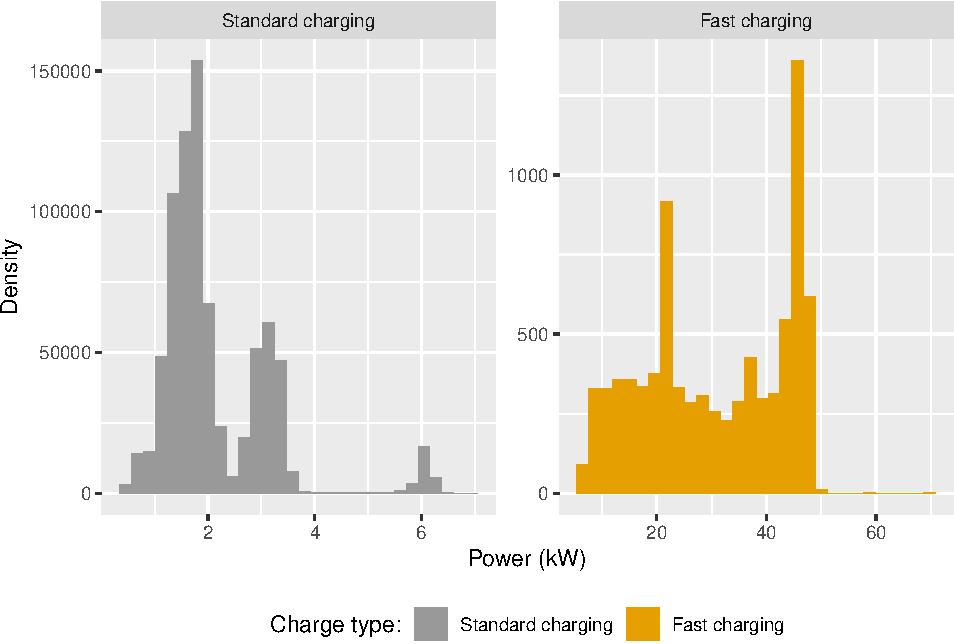
\includegraphics{EVBB_SummaryReport_files/figure-latex/obsPower-1.pdf}
\caption{\label{fig:obsPower}Observed power demand distribution by day of
the week and charge type where charging observed}
\end{figure}

\begin{Shaded}
\begin{Highlighting}[]
\NormalTok{stdQT <-}\StringTok{ }\KeywordTok{quantile}\NormalTok{(chargingDT[chargeType }\OperatorTok{==}\StringTok{ "Standard charging"}\NormalTok{]}\OperatorTok{$}\NormalTok{charge_power_kw)}
\NormalTok{fastQT <-}\StringTok{ }\KeywordTok{quantile}\NormalTok{(chargingDT[chargeType }\OperatorTok{==}\StringTok{ "Fast charging"}\NormalTok{]}\OperatorTok{$}\NormalTok{charge_power_kw)}
\end{Highlighting}
\end{Shaded}

75\% of standard charging observations were 1.46 kW or more but the
figure was 16.78 kW or more for fast charging

\section{Daily demand}\label{daily-demand}

\begin{Shaded}
\begin{Highlighting}[]
\NormalTok{p <-}\StringTok{ }\NormalTok{ggplot2}\OperatorTok{::}\KeywordTok{ggplot}\NormalTok{(}\KeywordTok{filter}\NormalTok{(dt, chargeType }\OperatorTok{==}\StringTok{ "Standard charging"} \OperatorTok{|}\StringTok{ }\NormalTok{chargeType }\OperatorTok{==}\StringTok{ "Fast charging"}\NormalTok{), }\KeywordTok{aes}\NormalTok{(}\DataTypeTok{x =}\NormalTok{ day_of_week, }\DataTypeTok{colour =}\NormalTok{ chargeType, }\DataTypeTok{group =}\NormalTok{ day_of_week)) }\OperatorTok{+}
\StringTok{  }\KeywordTok{geom_boxplot}\NormalTok{(}\KeywordTok{aes}\NormalTok{(}\DataTypeTok{y =}\NormalTok{ charge_power_kw)) }\OperatorTok{+}
\StringTok{  }\KeywordTok{facet_wrap}\NormalTok{(. }\OperatorTok{~}\StringTok{ }\NormalTok{chargeType, }\DataTypeTok{scales=} \StringTok{"free_y"}\NormalTok{)}

\NormalTok{p }\OperatorTok{+}\StringTok{ }\KeywordTok{theme}\NormalTok{(}\DataTypeTok{axis.text.x =} \KeywordTok{element_text}\NormalTok{(}\DataTypeTok{angle =} \DecValTok{90}\NormalTok{, }\DataTypeTok{hjust =} \DecValTok{1}\NormalTok{)) }\OperatorTok{+}\StringTok{ }
\StringTok{  }\KeywordTok{labs}\NormalTok{(}\DataTypeTok{x =} \StringTok{"Day of week"}\NormalTok{,}
       \DataTypeTok{y =} \StringTok{"Power (kW)"}\NormalTok{) }\OperatorTok{+}
\StringTok{  }\KeywordTok{guides}\NormalTok{(}\DataTypeTok{colour =} \KeywordTok{guide_legend}\NormalTok{(}\DataTypeTok{title =} \StringTok{"Charge type:"}\NormalTok{)) }\OperatorTok{+}
\StringTok{  }\KeywordTok{scale_colour_manual}\NormalTok{(}\DataTypeTok{values=}\NormalTok{cbgPalette) }\OperatorTok{+}\StringTok{ }\CommentTok{# use colour-blind friendly palette}
\StringTok{  }\KeywordTok{theme}\NormalTok{(}\DataTypeTok{legend.position =} \StringTok{"bottom"}\NormalTok{)}
\end{Highlighting}
\end{Shaded}

\begin{verbatim}
## Warning: Removed 45 rows containing non-finite values (stat_boxplot).
\end{verbatim}

\begin{figure}
\centering
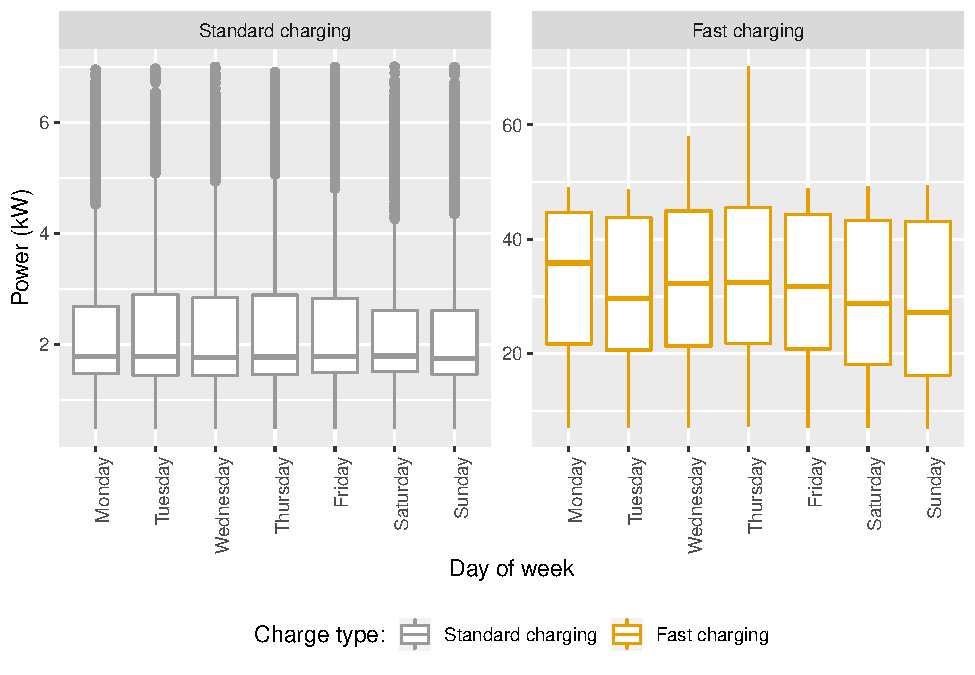
\includegraphics{EVBB_SummaryReport_files/figure-latex/dailyPower-1.pdf}
\caption{\label{fig:dailyPower}Observed power demand distribution by day of
the week and charge type}
\end{figure}

Figure \ref{fig:dailyPower} shows the distribution of observed charging
kW demand by day of the week. We can see that fast charging varies in
demand but standard charging is relatively constant across days.

\section{Charging duration}\label{duration}

Fig: Histogram of charging event durations (faceted by fast vs standard)

If we assume that the first non-zero charge observation is the `start'
and the last non-zero charge observation within the vehicle id is the
`end' we can calculate the duration between the two. This assumes there
is no missing data.

Figure \ref{fig:durationHist} shows the overall distribution of all
charging sequences. Clearly there are very small and a few very large
values for Standard Charges but this is not the case for Fast charges.

\begin{Shaded}
\begin{Highlighting}[]
\NormalTok{ggplot2}\OperatorTok{::}\KeywordTok{ggplot}\NormalTok{(firstLastDT[pairOK }\OperatorTok{==}\StringTok{ "Pair end"}\NormalTok{], }
                \KeywordTok{aes}\NormalTok{(}\DataTypeTok{x =}\NormalTok{ pairDurationFinal)) }\OperatorTok{+}
\StringTok{  }\KeywordTok{geom_histogram}\NormalTok{(}\DataTypeTok{binwidth =} \DecValTok{5}\NormalTok{) }\OperatorTok{+}
\StringTok{  }\KeywordTok{facet_wrap}\NormalTok{(chargeType }\OperatorTok{~}\StringTok{ }\NormalTok{., }\DataTypeTok{scales =} \StringTok{"free"}\NormalTok{) }\OperatorTok{+}
\StringTok{  }\KeywordTok{labs}\NormalTok{(}\DataTypeTok{x =} \StringTok{"Minutes"}\NormalTok{)}
\end{Highlighting}
\end{Shaded}

\begin{figure}
\centering
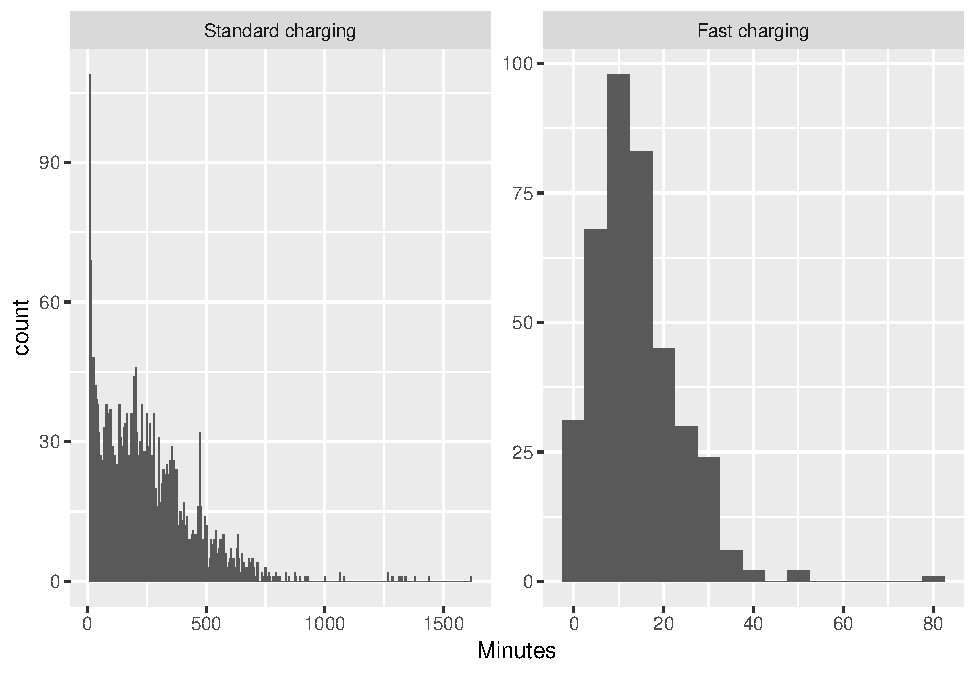
\includegraphics{EVBB_SummaryReport_files/figure-latex/durationHist-1.pdf}
\caption{\label{fig:durationHist}Duration of charging sequences}
\end{figure}

Table \ref{tab:durationDescTable} shows the overall distributions and
indicates the extent to which the means are skewed by the very small and
a few very large values shown in Figure \ref{fig:durationHist}.

\begin{Shaded}
\begin{Highlighting}[]
\NormalTok{t <-}\StringTok{ }\NormalTok{firstLastDT[pairOK }\OperatorTok{==}\StringTok{ "Pair end"}\NormalTok{, }
\NormalTok{                 .(}\DataTypeTok{N =}\NormalTok{ .N,}
                   \DataTypeTok{mean =} \KeywordTok{mean}\NormalTok{(pairDurationFinal),}
                   \DataTypeTok{median =} \KeywordTok{median}\NormalTok{(pairDurationFinal),}
                   \DataTypeTok{min =} \KeywordTok{min}\NormalTok{(pairDurationFinal),}
                   \DataTypeTok{max =} \KeywordTok{max}\NormalTok{(pairDurationFinal)), }
\NormalTok{                 keyby =}\StringTok{ }\NormalTok{.(chargeType)]}
\NormalTok{kableExtra}\OperatorTok{::}\KeywordTok{kable}\NormalTok{(t, }
                  \DataTypeTok{caption =} \StringTok{"Duration of all charge sequences by charge type (minutes)"}\NormalTok{, }\DataTypeTok{digits =} \DecValTok{2}\NormalTok{) }\OperatorTok
\StringTok{  }\KeywordTok{kable_styling}\NormalTok{()}
\end{Highlighting}
\end{Shaded}

\begin{table}[t]

\caption{\label{tab:durationDescTable}Duration of all charge sequences by charge type (minutes)}
\centering
\begin{tabular}{l|r|r|r|r|r}
\hline
chargeType & N & mean & median & min & max\\
\hline
Standard charging & 8584 & 82.58 & 3.43 & 0.27 & 876.67\\
\hline
Fast charging & 593 & 13.03 & 11.88 & 0.32 & 48.78\\
\hline
\end{tabular}
\end{table}

Figure \ref{fig:shortDuration} shows the distribution of very short
charging sequences which are likely to be `top-ups' occuring towards the
end of a longer charging period. As we can see these appear to be
generally less than 8 minutes in length for Standard Charges.

\begin{Shaded}
\begin{Highlighting}[]
\NormalTok{ggplot2}\OperatorTok{::}\KeywordTok{ggplot}\NormalTok{(firstLastDT[pairOK }\OperatorTok{==}\StringTok{ "Pair end"} \OperatorTok{&}\StringTok{ }\NormalTok{pairDurationFinal }\OperatorTok{<}\StringTok{ }\DecValTok{10}\NormalTok{], }
                \KeywordTok{aes}\NormalTok{(}\DataTypeTok{x =}\NormalTok{ pairDurationFinal)) }\OperatorTok{+}
\StringTok{  }\KeywordTok{geom_histogram}\NormalTok{(}\DataTypeTok{binwidth =} \DecValTok{1}\NormalTok{) }\OperatorTok{+}
\StringTok{  }\KeywordTok{facet_grid}\NormalTok{(chargeType }\OperatorTok{~}\StringTok{ }\NormalTok{.) }\OperatorTok{+}
\StringTok{  }\KeywordTok{labs}\NormalTok{(}\DataTypeTok{x =} \StringTok{"Minutes"}\NormalTok{)}
\end{Highlighting}
\end{Shaded}

\begin{figure}
\centering
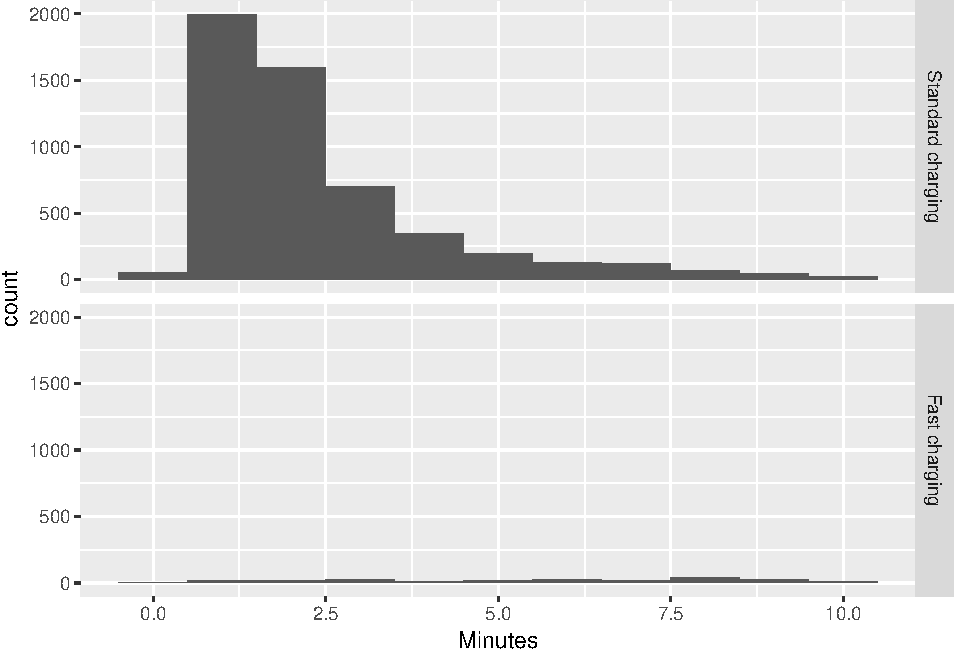
\includegraphics{EVBB_SummaryReport_files/figure-latex/shortDuration-1.pdf}
\caption{\label{fig:shortDuration}Duration of charging sequences \textless{}
10 minutes}
\end{figure}

Table \ref{tab:durationDescTableReduced} shows the same descriptive
statistics but for all sequences of greater than 8 minute duration. Now
we can see that the mean and median durations for Standard Charge
sequences are closer at 130 - 140 minutes.

\begin{Shaded}
\begin{Highlighting}[]
\NormalTok{t <-}\StringTok{ }\NormalTok{firstLastDT[pairOK }\OperatorTok{==}\StringTok{ "Pair end"} \OperatorTok{&}\StringTok{ }\NormalTok{pairDurationFinal }\OperatorTok{>}\StringTok{ }\DecValTok{8}\NormalTok{, }
\NormalTok{                 .(}\DataTypeTok{N =}\NormalTok{ .N,}
                   \DataTypeTok{mean =} \KeywordTok{mean}\NormalTok{(pairDurationFinal),}
                   \DataTypeTok{median =} \KeywordTok{median}\NormalTok{(pairDurationFinal),}
                   \DataTypeTok{min =} \KeywordTok{min}\NormalTok{(pairDurationFinal),}
                   \DataTypeTok{max =} \KeywordTok{max}\NormalTok{(pairDurationFinal)), }
\NormalTok{                 keyby =}\StringTok{ }\NormalTok{.(chargeType)]}
\NormalTok{kableExtra}\OperatorTok{::}\KeywordTok{kable}\NormalTok{(t, }
                  \DataTypeTok{caption =} \StringTok{"Duration of charge sequences > 8 minutes by charge type (minutes, )"}\NormalTok{, }\DataTypeTok{digits =} \DecValTok{2}\NormalTok{) }\OperatorTok
\StringTok{  }\KeywordTok{kable_styling}\NormalTok{()}
\end{Highlighting}
\end{Shaded}

\begin{table}[t]

\caption{\label{tab:durationDescTableReduced}Duration of charge sequences > 8 minutes by charge type (minutes, )}
\centering
\begin{tabular}{l|r|r|r|r|r}
\hline
chargeType & N & mean & median & min & max\\
\hline
Standard charging & 3402 & 204.99 & 176.64 & 8.02 & 876.67\\
\hline
Fast charging & 417 & 16.64 & 15.18 & 8.05 & 48.78\\
\hline
\end{tabular}
\end{table}

Figure \ref{fig:longDuration} shows the distribution of long
(\textgreater{} 8 minutes) charging sequences. As we can see these
appear to be generally less than 3 hours in length for Standard Charges.

\begin{Shaded}
\begin{Highlighting}[]
\NormalTok{ggplot2}\OperatorTok{::}\KeywordTok{ggplot}\NormalTok{(firstLastDT[pairOK }\OperatorTok{==}\StringTok{ "Pair end"} \OperatorTok{&}\StringTok{ }\NormalTok{pairDurationFinal }\OperatorTok{>}\StringTok{ }\DecValTok{8} \OperatorTok{&}\StringTok{ }\NormalTok{pairDurationFinal }\OperatorTok{<}\StringTok{ }\DecValTok{6000}\NormalTok{], }
                \KeywordTok{aes}\NormalTok{(}\DataTypeTok{x =}\NormalTok{ pairDurationFinal)) }\OperatorTok{+}
\StringTok{  }\KeywordTok{geom_histogram}\NormalTok{(}\DataTypeTok{binwidth =} \DecValTok{20}\NormalTok{) }\OperatorTok{+}
\StringTok{  }\KeywordTok{facet_grid}\NormalTok{(chargeType }\OperatorTok{~}\StringTok{ }\NormalTok{., }\DataTypeTok{scales =} \StringTok{"free"}\NormalTok{) }\OperatorTok{+}
\StringTok{  }\KeywordTok{labs}\NormalTok{(}\DataTypeTok{x =} \StringTok{"Minutes"}\NormalTok{)}
\end{Highlighting}
\end{Shaded}

\begin{figure}
\centering
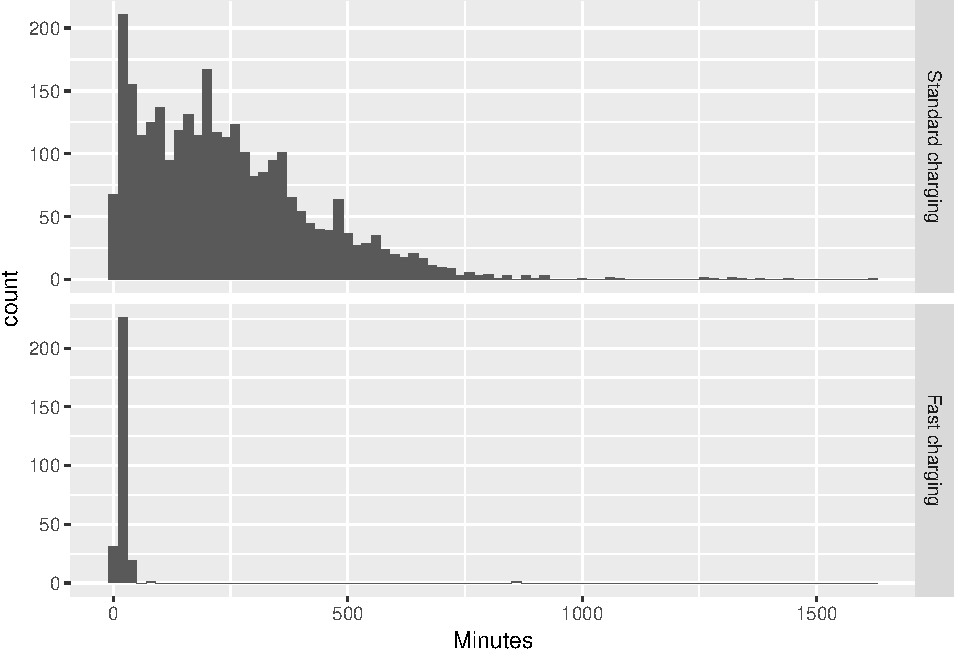
\includegraphics{EVBB_SummaryReport_files/figure-latex/longDuration-1.pdf}
\caption{\label{fig:longDuration}Duration of charging sequences
\textgreater{} 8 minutes}
\end{figure}

\subsection{Duration by time of day}\label{duration-by-time-of-day}

\begin{Shaded}
\begin{Highlighting}[]
\NormalTok{ggplot2}\OperatorTok{::}\KeywordTok{ggplot}\NormalTok{(firstLastDT[pairOK }\OperatorTok{==}\StringTok{ "Pair end"} \OperatorTok{&}\StringTok{ }\NormalTok{pairDurationFinal }\OperatorTok{>}\StringTok{ }\DecValTok{8} \OperatorTok{&}\StringTok{ }\NormalTok{pairDurationFinal }\OperatorTok{<}\StringTok{ }\DecValTok{6000}\NormalTok{], }
                \KeywordTok{aes}\NormalTok{(}\DataTypeTok{x =}\NormalTok{ qHour, }\DataTypeTok{y =}\NormalTok{ pairDurationFinal, }\DataTypeTok{group =}\NormalTok{ qHour)) }\OperatorTok{+}
\StringTok{  }\KeywordTok{geom_boxplot}\NormalTok{() }\OperatorTok{+}
\StringTok{  }\KeywordTok{facet_grid}\NormalTok{(chargeType }\OperatorTok{~}\StringTok{ }\NormalTok{., }\DataTypeTok{scales =} \StringTok{"free"}\NormalTok{) }\OperatorTok{+}
\StringTok{  }\KeywordTok{labs}\NormalTok{(}\DataTypeTok{x =} \StringTok{"Time of Day"}\NormalTok{,}
       \DataTypeTok{y =} \StringTok{"Minutes"}\NormalTok{)}
\end{Highlighting}
\end{Shaded}

\begin{figure}
\centering
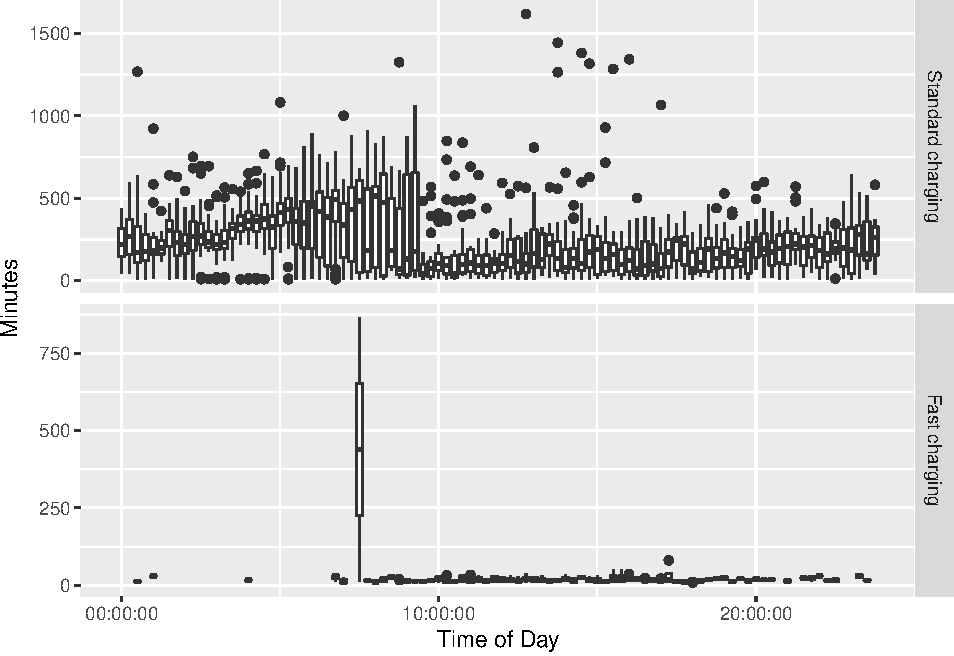
\includegraphics{EVBB_SummaryReport_files/figure-latex/durationTimeBox-1.pdf}
\caption{\label{fig:durationTimeBox}Duration by time of charging start for
sequences \textgreater{} 8 minutes}
\end{figure}

\begin{Shaded}
\begin{Highlighting}[]
\NormalTok{plotDT <-}\StringTok{ }\NormalTok{firstLastDT[pairOK }\OperatorTok{==}\StringTok{ "Pair end"} \OperatorTok{&}\StringTok{ }\NormalTok{pairDurationFinal }\OperatorTok{>}\StringTok{ }\DecValTok{8}\NormalTok{,}
\NormalTok{                      .(}\DataTypeTok{meanDuration =} \KeywordTok{mean}\NormalTok{(pairDurationFinal)),}
\NormalTok{                      keyby =}\StringTok{ }\NormalTok{.(qHour, chargeType)]}
\NormalTok{ggplot2}\OperatorTok{::}\KeywordTok{ggplot}\NormalTok{(plotDT, }
                \KeywordTok{aes}\NormalTok{(}\DataTypeTok{x =}\NormalTok{ qHour, }\DataTypeTok{y =}\NormalTok{ meanDuration, }\DataTypeTok{colour =}\NormalTok{ chargeType)) }\OperatorTok{+}
\StringTok{  }\KeywordTok{geom_point}\NormalTok{() }\OperatorTok{+}
\StringTok{  }\KeywordTok{labs}\NormalTok{(}\DataTypeTok{x =} \StringTok{"Time of Day"}\NormalTok{,}
       \DataTypeTok{y =} \StringTok{"Minutes"}\NormalTok{)}
\end{Highlighting}
\end{Shaded}

\begin{figure}
\centering
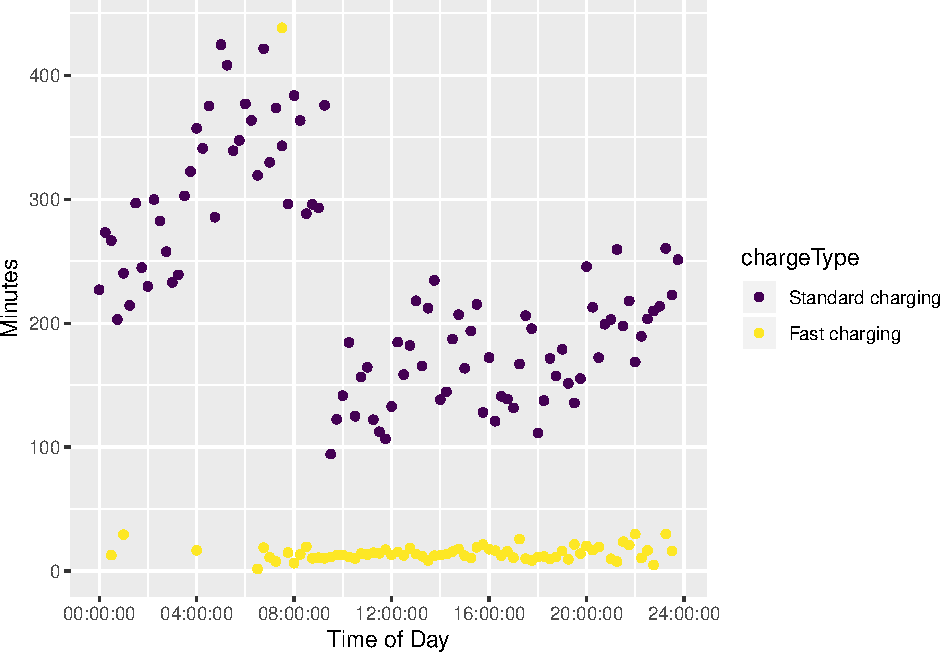
\includegraphics{EVBB_SummaryReport_files/figure-latex/durationTimeMean-1.pdf}
\caption{\label{fig:durationTimeMean}Mean duration (within quarter hours) by
time of charging start for sequences \textgreater{} 8 minutes}
\end{figure}

\begin{Shaded}
\begin{Highlighting}[]
\NormalTok{kableExtra}\OperatorTok{::}\KeywordTok{kable}\NormalTok{(t, }\DataTypeTok{caption =} \StringTok{"Mean duration of charge events by charge type"}\NormalTok{)}
\end{Highlighting}
\end{Shaded}

\begin{table}[t]

\caption{\label{tab:meanDurationTable}Mean duration of charge events by charge type}
\centering
\begin{tabular}{l|r|r|r|r|r}
\hline
chargeType & N & mean & median & min & max\\
\hline
Standard charging & 3402 & 204.99240 & 176.64167 & 8.016667 & 876.66667\\
\hline
Fast charging & 417 & 16.63513 & 15.18333 & 8.050000 & 48.78333\\
\hline
\end{tabular}
\end{table}

\begin{Shaded}
\begin{Highlighting}[]
\NormalTok{plotDT <-}\StringTok{ }\NormalTok{firstLastDT[pairOK }\OperatorTok{==}\StringTok{ "Pair end"}\NormalTok{, .(}\DataTypeTok{meanDuration =} \KeywordTok{mean}\NormalTok{(pairDurationFinal, }\DataTypeTok{na.rm =} \OtherTok{TRUE}\NormalTok{)), keyby =}\StringTok{ }\NormalTok{.(chargeType, dateTime)]}
\end{Highlighting}
\end{Shaded}

\begin{quote}
Discuss any other patterns
\end{quote}

\begin{quote}
What was the research question? :-)
\end{quote}

\section{Time of charging}\label{time-of-charging}

\begin{Shaded}
\begin{Highlighting}[]
\NormalTok{plotDT <-}\StringTok{ }\NormalTok{chargingDT[, .(}\DataTypeTok{count =}\NormalTok{ .N), keyby =}\StringTok{ }\NormalTok{.(qHour, chargeType, day_of_week)]}

\CommentTok{# make a weekend facet label}
\NormalTok{plotDT <-}\StringTok{ }\NormalTok{plotDT[, weekEnd }\OperatorTok{:}\ErrorTok{=}\StringTok{ "Weekend"}\NormalTok{]}
\NormalTok{plotDT <-}\StringTok{ }\NormalTok{plotDT[day_of_week }\OperatorTok{!=}\StringTok{ "Saturday"} \OperatorTok{&}\StringTok{ }\NormalTok{day_of_week }\OperatorTok{!=}\StringTok{ "Sunday"}\NormalTok{, weekEnd }\OperatorTok{:}\ErrorTok{=}\StringTok{ "Week day"}\NormalTok{]}

\NormalTok{p <-}\StringTok{ }\NormalTok{ggplot2}\OperatorTok{::}\KeywordTok{ggplot}\NormalTok{(plotDT, }\KeywordTok{aes}\NormalTok{(}\DataTypeTok{x =}\NormalTok{ qHour, }\DataTypeTok{y =}\NormalTok{ count, }\DataTypeTok{colour =}\NormalTok{ day_of_week)) }\OperatorTok{+}
\StringTok{  }\KeywordTok{geom_line}\NormalTok{() }\OperatorTok{+}
\StringTok{  }\KeywordTok{facet_grid}\NormalTok{(weekEnd }\OperatorTok{~}\StringTok{  }\NormalTok{chargeType, }\DataTypeTok{scales =} \StringTok{"free_y"}\NormalTok{)}
  
\NormalTok{p }\OperatorTok{+}\StringTok{ }\KeywordTok{theme}\NormalTok{(}\DataTypeTok{axis.text.x =} \KeywordTok{element_text}\NormalTok{(}\DataTypeTok{angle =} \DecValTok{90}\NormalTok{, }\DataTypeTok{hjust =} \DecValTok{1}\NormalTok{)) }\OperatorTok{+}\StringTok{ }
\StringTok{  }\KeywordTok{labs}\NormalTok{(}\DataTypeTok{x =} \StringTok{"Time of day"}\NormalTok{,}
       \DataTypeTok{y =} \StringTok{"Count"}\NormalTok{) }\OperatorTok{+}
\StringTok{  }\KeywordTok{guides}\NormalTok{(}\DataTypeTok{colour =} \KeywordTok{guide_legend}\NormalTok{(}\DataTypeTok{title =} \StringTok{"Day of week:"}\NormalTok{)) }\OperatorTok{+}
\StringTok{  }\KeywordTok{scale_colour_manual}\NormalTok{(}\DataTypeTok{values=}\NormalTok{cbgPalette) }\OperatorTok{+}\StringTok{ }\CommentTok{# use colour-blind friendly palette}
\StringTok{  }\KeywordTok{theme}\NormalTok{(}\DataTypeTok{legend.position =} \StringTok{"bottom"}\NormalTok{)}
\end{Highlighting}
\end{Shaded}

\begin{figure}
\centering
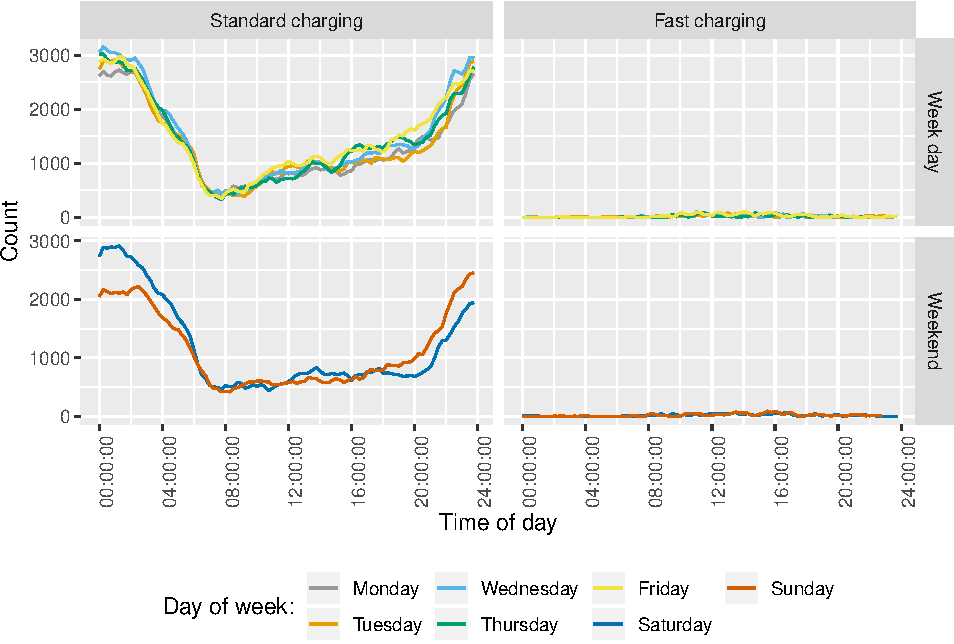
\includegraphics{EVBB_SummaryReport_files/figure-latex/chargeTime-1.pdf}
\caption{\label{fig:chargeTime}Count of observed charging events by type,
day of week and time}
\end{figure}

Figure \ref{fig:chargeTime} shows the distribution of observed charging
by time of day and day of the week. Aggregating counts in this way
emphasises the times at which charging most commonly occurs and we can
see\ldots{}

Fig: profile of median charging demand by time of day and day of the
week faceted by at home vs not at home

Charging demand varies somewhat by time of day and day of the week.
Weekdays show \ldots{} whilst weekends show. Saturdays and Sundays vary
with\ldots{}

\begin{Shaded}
\begin{Highlighting}[]
\NormalTok{p <-}\StringTok{ }\NormalTok{ggplot2}\OperatorTok{::}\KeywordTok{ggplot}\NormalTok{(}\KeywordTok{subset}\NormalTok{(df, chargeType }\OperatorTok\StringTok{ "Standard charging"}\NormalTok{), }
                     \KeywordTok{aes}\NormalTok{(}\DataTypeTok{x =}\NormalTok{ qHour, }\DataTypeTok{group =}\NormalTok{ qHour, }\DataTypeTok{y =}\NormalTok{ charge_power_kw)) }\OperatorTok{+}
\StringTok{  }\KeywordTok{theme}\NormalTok{(}\DataTypeTok{legend.position =} \StringTok{"bottom"}\NormalTok{, }\DataTypeTok{axis.text.x =} \KeywordTok{element_text}\NormalTok{(}\DataTypeTok{angle =} \DecValTok{90}\NormalTok{)) }\OperatorTok{+}
\StringTok{  }\KeywordTok{scale_colour_manual}\NormalTok{(}\DataTypeTok{values=}\NormalTok{cbbPalette) }\OperatorTok{+}\StringTok{ }\CommentTok{# use colour-blind friendly palette}
\StringTok{  }\KeywordTok{geom_boxplot}\NormalTok{() }\CommentTok{# <- make the plot in an object first}

\NormalTok{p }\OperatorTok{+}\StringTok{ }\KeywordTok{labs}\NormalTok{(}\DataTypeTok{x =} \StringTok{"Time of Day"}\NormalTok{, }\DataTypeTok{y =} \StringTok{"Power (kW)"}\NormalTok{, }\DataTypeTok{caption =} \StringTok{"Boxplot of daily standard charging demand"}\NormalTok{)}
\end{Highlighting}
\end{Shaded}

\begin{figure}
\centering
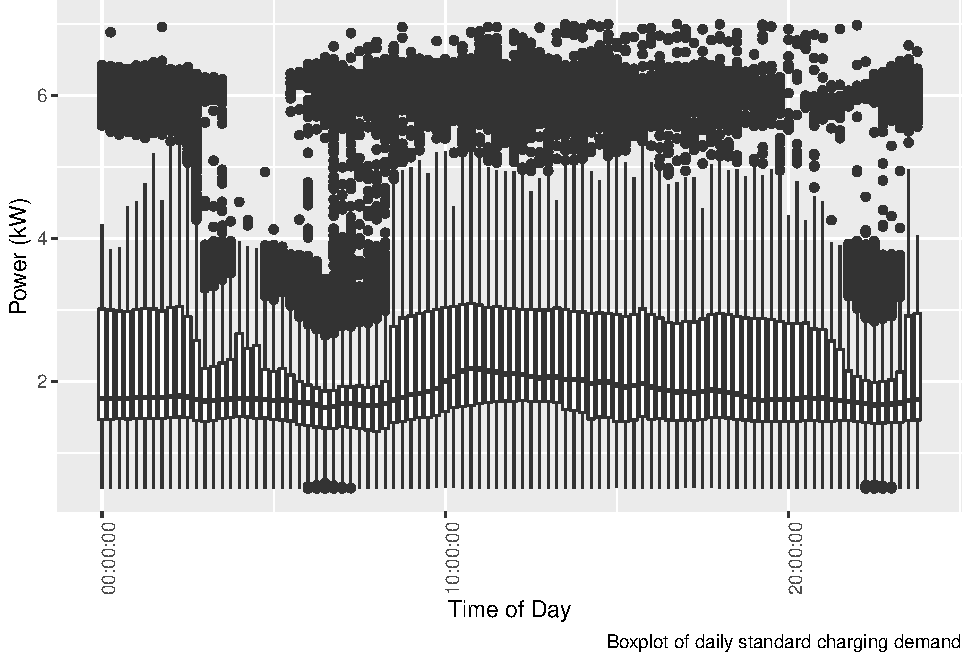
\includegraphics{EVBB_SummaryReport_files/figure-latex/boxplotCharging-1.pdf}
\caption{\label{fig:boxplotCharging}Boxplot of charging timing by charge
rate}
\end{figure}

\begin{Shaded}
\begin{Highlighting}[]
\KeywordTok{ggplot}\NormalTok{(df,}\KeywordTok{aes}\NormalTok{(}\DataTypeTok{x=}\NormalTok{charge_power_kw, }\DataTypeTok{y=}\NormalTok{forcats}\OperatorTok{::}\KeywordTok{fct_rev}\NormalTok{(day_of_week))) }\OperatorTok{+}
\StringTok{  }\KeywordTok{geom_density_ridges}\NormalTok{(}\DataTypeTok{rel_min_height =} \FloatTok{0.01}\NormalTok{) }\OperatorTok{+}\StringTok{        }\CommentTok{# removes tails}
\StringTok{  }\KeywordTok{scale_x_discrete}\NormalTok{(}\DataTypeTok{expand =} \KeywordTok{c}\NormalTok{(}\FloatTok{0.01}\NormalTok{, }\DecValTok{0}\NormalTok{)) }\OperatorTok{+}\StringTok{  }\CommentTok{# removes cutoff top}
\StringTok{  }\KeywordTok{labs}\NormalTok{(}\DataTypeTok{x=}\StringTok{"Charging power"}\NormalTok{,}\DataTypeTok{y=}\StringTok{"Day"}\NormalTok{)}
\end{Highlighting}
\end{Shaded}

\begin{verbatim}
## Picking joint bandwidth of 0.11
\end{verbatim}

\begin{verbatim}
## Warning: Removed 45 rows containing non-finite values
## (stat_density_ridges).
\end{verbatim}

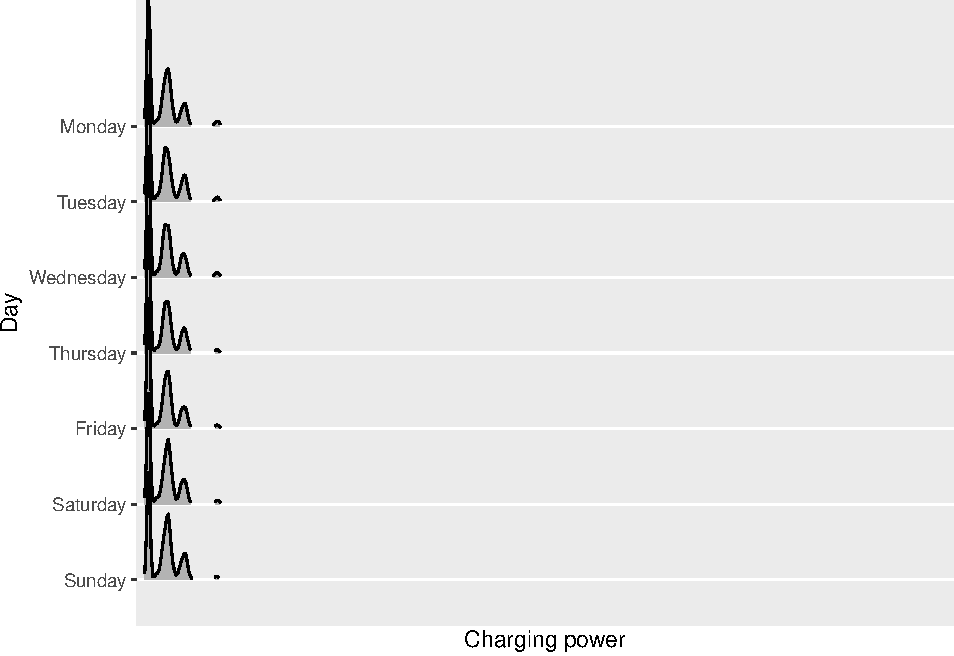
\includegraphics{EVBB_SummaryReport_files/figure-latex/joyplot-1.pdf}

\begin{Shaded}
\begin{Highlighting}[]
\NormalTok{p <-}\StringTok{ }\NormalTok{ggplot2}\OperatorTok{::}\KeywordTok{ggplot}\NormalTok{(}\KeywordTok{subset}\NormalTok{(dt, chargeType }\OperatorTok\StringTok{ "Fast charging"}\NormalTok{), }
                     \KeywordTok{aes}\NormalTok{(}\DataTypeTok{x =}\NormalTok{ qHour, }\DataTypeTok{group =}\NormalTok{ qHour, }\DataTypeTok{y =}\NormalTok{ charge_power_kw)) }\OperatorTok{+}
\StringTok{  }\KeywordTok{theme}\NormalTok{(}\DataTypeTok{legend.position =} \StringTok{"bottom"}\NormalTok{, }\DataTypeTok{axis.text.x =} \KeywordTok{element_text}\NormalTok{(}\DataTypeTok{angle =} \DecValTok{90}\NormalTok{)) }\OperatorTok{+}
\StringTok{  }\KeywordTok{scale_colour_manual}\NormalTok{(}\DataTypeTok{values=}\NormalTok{cbbPalette) }\OperatorTok{+}\StringTok{ }\CommentTok{# use colour-blind friendly palette}
\StringTok{  }\KeywordTok{geom_boxplot}\NormalTok{() }\CommentTok{# <- make the plot in an object first}

\NormalTok{p }\OperatorTok{+}\StringTok{ }\KeywordTok{labs}\NormalTok{(}\DataTypeTok{x =} \StringTok{"Time of Day"}\NormalTok{, }\DataTypeTok{y =} \StringTok{"Power (kW)"}\NormalTok{, }\DataTypeTok{caption =} \StringTok{"Boxplot of daily fast charging demand"}\NormalTok{)}
\end{Highlighting}
\end{Shaded}

\begin{verbatim}
## Warning: Removed 45 rows containing non-finite values (stat_boxplot).
\end{verbatim}

\begin{figure}
\centering
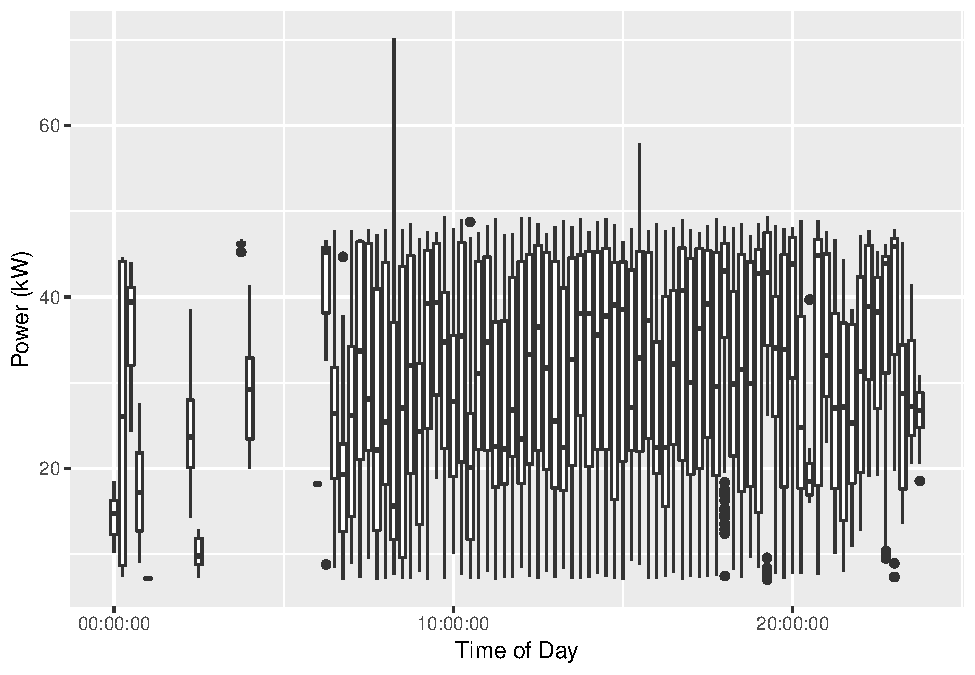
\includegraphics{EVBB_SummaryReport_files/figure-latex/plot3-1.pdf}
\caption{\label{fig:plot3}Boxplot of charging timing by charge rate}
\end{figure}

\begin{Shaded}
\begin{Highlighting}[]
\NormalTok{p <-}\StringTok{ }\NormalTok{ggplot2}\OperatorTok{::}\KeywordTok{ggplot}\NormalTok{(dt, }\KeywordTok{aes}\NormalTok{(}\DataTypeTok{x =}\NormalTok{ qHour, }\DataTypeTok{group =}\NormalTok{ qHour, }\DataTypeTok{y =}\NormalTok{ charge_power_kw)) }\OperatorTok{+}
\StringTok{  }\KeywordTok{guides}\NormalTok{(}\DataTypeTok{colour =} \KeywordTok{guide_legend}\NormalTok{(}\DataTypeTok{title =} \StringTok{"Vehicle:"}\NormalTok{)) }\OperatorTok{+}
\StringTok{  }\KeywordTok{theme}\NormalTok{(}\DataTypeTok{legend.position =} \StringTok{"bottom"}\NormalTok{, }\DataTypeTok{axis.text.x =} \KeywordTok{element_text}\NormalTok{(}\DataTypeTok{angle =} \DecValTok{90}\NormalTok{)) }\OperatorTok{+}
\StringTok{  }\KeywordTok{scale_colour_manual}\NormalTok{(}\DataTypeTok{values=}\NormalTok{cbbPalette) }\OperatorTok{+}\StringTok{ }
\StringTok{  }\KeywordTok{geom_boxplot}\NormalTok{() }

\NormalTok{p }\OperatorTok{+}\StringTok{ }\KeywordTok{labs}\NormalTok{(}\DataTypeTok{x =} \StringTok{"Time of Day"}\NormalTok{, }\DataTypeTok{y =} \StringTok{"Power (kW)"}\NormalTok{)}
\end{Highlighting}
\end{Shaded}

\begin{verbatim}
## Warning: Removed 45 rows containing non-finite values (stat_boxplot).
\end{verbatim}

\begin{figure}
\centering
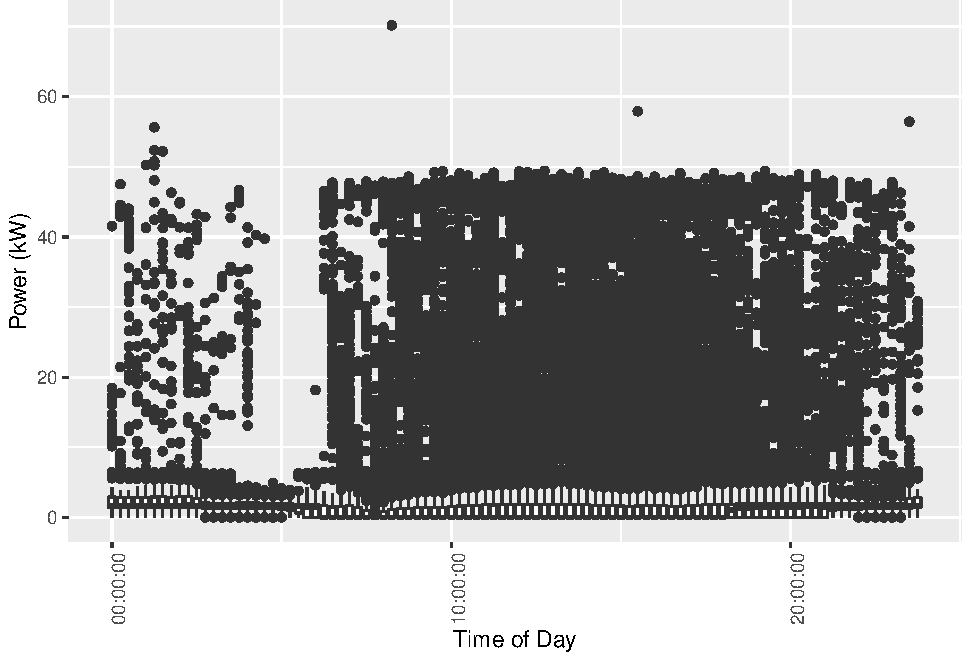
\includegraphics{EVBB_SummaryReport_files/figure-latex/plot2-1.pdf}
\caption{\label{fig:plot2}Boxplot of charging timing}
\end{figure}

\begin{Shaded}
\begin{Highlighting}[]
\KeywordTok{ggplot}\NormalTok{(chargeBegins,}\KeywordTok{aes}\NormalTok{(}\DataTypeTok{x=}\NormalTok{qHour, }\DataTypeTok{y=}\NormalTok{ forcats}\OperatorTok{::}\KeywordTok{fct_rev}\NormalTok{(day_of_week))) }\OperatorTok{+}
\StringTok{  }\KeywordTok{geom_density_ridges}\NormalTok{(}\DataTypeTok{rel_min_height =} \FloatTok{0.01}\NormalTok{) }\OperatorTok{+}\StringTok{        }\CommentTok{# removes tails}
\StringTok{  }\KeywordTok{scale_x_discrete}\NormalTok{(}\DataTypeTok{expand =} \KeywordTok{c}\NormalTok{(}\FloatTok{0.01}\NormalTok{, }\DecValTok{0}\NormalTok{)) }\OperatorTok{+}\StringTok{  }\CommentTok{# removes cutoff top}
\StringTok{  }\KeywordTok{labs}\NormalTok{(}\DataTypeTok{x =} \StringTok{"Hour"}\NormalTok{, }\DataTypeTok{y =} \StringTok{"Day"}\NormalTok{) }
\end{Highlighting}
\end{Shaded}

\begin{verbatim}
## Picking joint bandwidth of 5700
\end{verbatim}

\begin{figure}
\centering
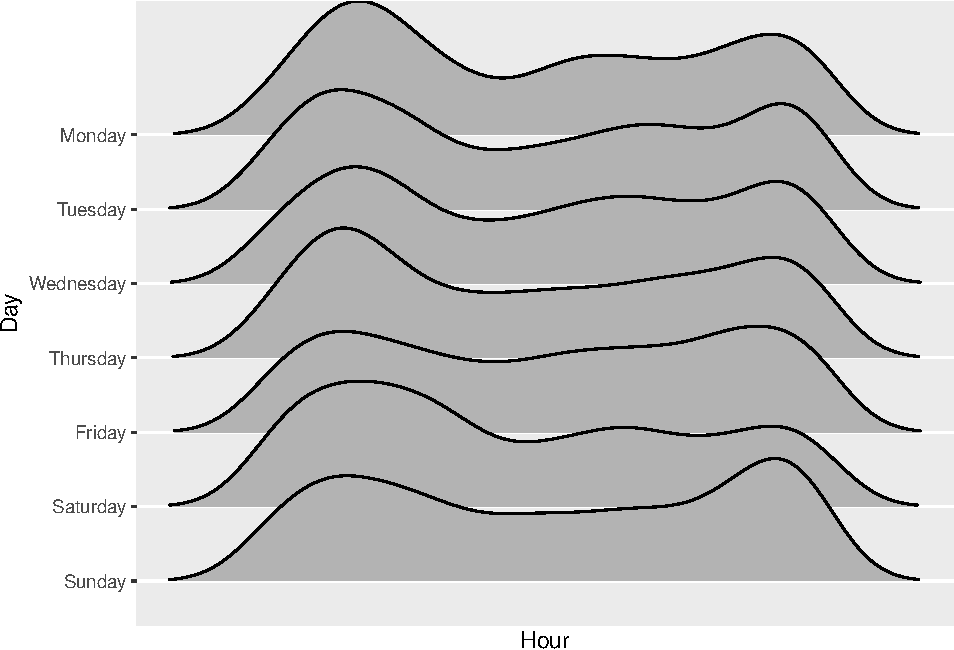
\includegraphics{EVBB_SummaryReport_files/figure-latex/ggjoyplotTimeChargingBegins-1.pdf}
\caption{\label{fig:ggjoyplotTimeChargingBegins}Time charging begins}
\end{figure}

\begin{Shaded}
\begin{Highlighting}[]
\CommentTok{# Not sure how to get time on x axis (or if I want to)}
\CommentTok{# ATTN BEN I don't think this joy plot gives any more information than we get from the following 2 density plots. Delete this entire block if you agree.}
\end{Highlighting}
\end{Shaded}

\begin{Shaded}
\begin{Highlighting}[]
\NormalTok{p <-}\StringTok{ }\KeywordTok{ggplot}\NormalTok{(chargeBegins[chargeBegins}\OperatorTok{$}\NormalTok{weekday }\OperatorTok{==}\StringTok{ "Weekday"}\NormalTok{, ], }\KeywordTok{aes}\NormalTok{(}\DataTypeTok{x =}\NormalTok{ qHour, }\DataTypeTok{fill =}\NormalTok{ chargeType)) }\OperatorTok{+}
\StringTok{  }\KeywordTok{geom_density}\NormalTok{(}\DataTypeTok{alpha =} \FloatTok{0.3}\NormalTok{) }
  \KeywordTok{facet_grid}\NormalTok{(}\OperatorTok{~}\NormalTok{weekday)}
\end{Highlighting}
\end{Shaded}

\begin{verbatim}
## <ggproto object: Class FacetGrid, Facet, gg>
##     compute_layout: function
##     draw_back: function
##     draw_front: function
##     draw_labels: function
##     draw_panels: function
##     finish_data: function
##     init_scales: function
##     map_data: function
##     params: list
##     setup_data: function
##     setup_params: function
##     shrink: TRUE
##     train_scales: function
##     vars: function
##     super:  <ggproto object: Class FacetGrid, Facet, gg>
\end{verbatim}

\begin{Shaded}
\begin{Highlighting}[]
\NormalTok{p }\OperatorTok{+}\StringTok{ }\KeywordTok{labs}\NormalTok{(}\DataTypeTok{x =} \StringTok{"Time"}\NormalTok{, }\DataTypeTok{fill =} \StringTok{"Charge type"}\NormalTok{)}
\end{Highlighting}
\end{Shaded}

\begin{figure}
\centering
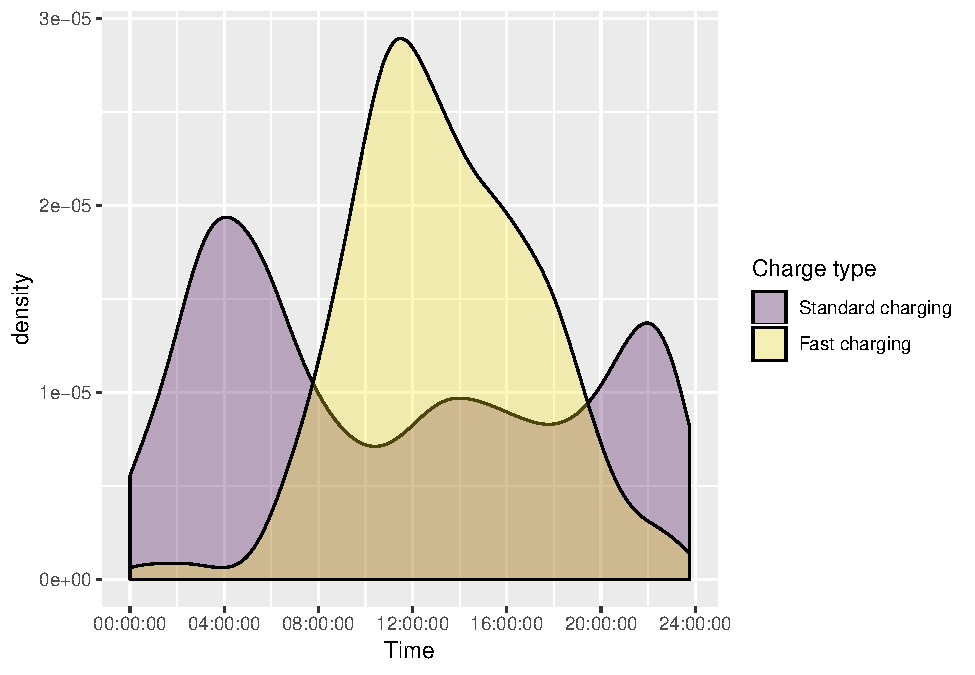
\includegraphics{EVBB_SummaryReport_files/figure-latex/chargeBeginsWeekday-1.pdf}
\caption{\label{fig:chargeBeginsWeekday}Density plot of charging start times
during weekdays}
\end{figure}

\begin{Shaded}
\begin{Highlighting}[]
\NormalTok{p <-}\StringTok{ }\KeywordTok{ggplot}\NormalTok{(chargeBegins[chargeBegins}\OperatorTok{$}\NormalTok{weekday }\OperatorTok{==}\StringTok{ "Weekend"}\NormalTok{, ], }\KeywordTok{aes}\NormalTok{(}\DataTypeTok{x =}\NormalTok{ qHour, }\DataTypeTok{fill =}\NormalTok{ chargeType)) }\OperatorTok{+}
\StringTok{  }\KeywordTok{geom_density}\NormalTok{(}\DataTypeTok{alpha =} \FloatTok{0.3}\NormalTok{) }
\NormalTok{p }\OperatorTok{+}\StringTok{ }\KeywordTok{labs}\NormalTok{(}\DataTypeTok{x =} \StringTok{"Time"}\NormalTok{, }\DataTypeTok{fill =} \StringTok{"Charge type"}\NormalTok{)}
\end{Highlighting}
\end{Shaded}

\begin{figure}
\centering
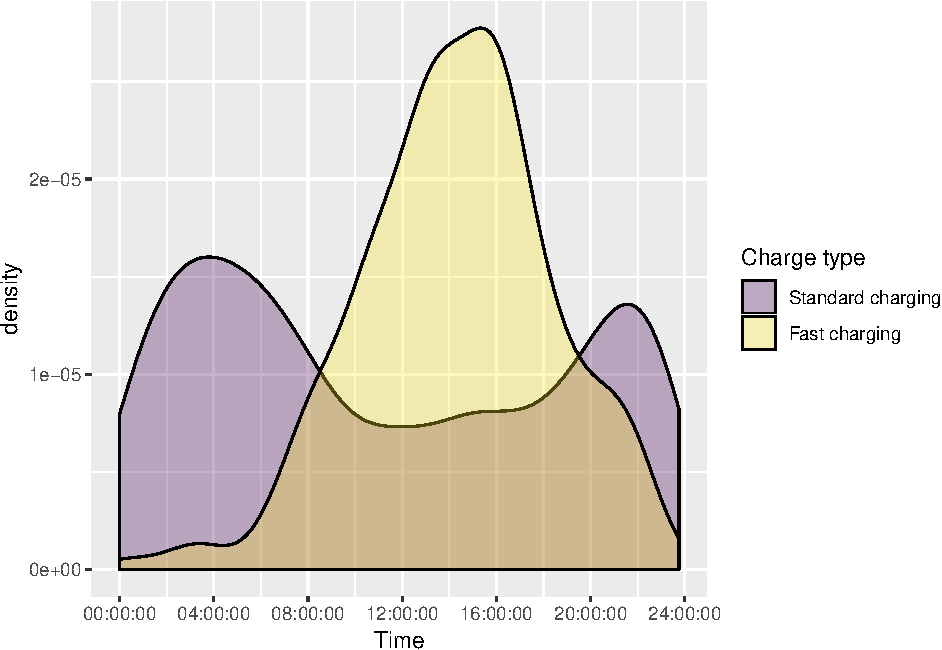
\includegraphics{EVBB_SummaryReport_files/figure-latex/chargeBeginsWeekend-1.pdf}
\caption{\label{fig:chargeBeginsWeekend}Density plot of charging start times
during weekends}
\end{figure}

\begin{Shaded}
\begin{Highlighting}[]
\NormalTok{p <-}\StringTok{ }\KeywordTok{ggplot}\NormalTok{(chargeEnds[chargeEnds}\OperatorTok{$}\NormalTok{weekday }\OperatorTok{==}\StringTok{ "Weekday"}\NormalTok{, ], }\KeywordTok{aes}\NormalTok{(}\DataTypeTok{x =}\NormalTok{ qHour, }\DataTypeTok{fill =}\NormalTok{ chargeType)) }\OperatorTok{+}
\StringTok{  }\KeywordTok{geom_density}\NormalTok{(}\DataTypeTok{alpha =} \FloatTok{0.3}\NormalTok{) }
\NormalTok{p }\OperatorTok{+}\StringTok{ }\KeywordTok{labs}\NormalTok{(}\DataTypeTok{x =} \StringTok{"Time"}\NormalTok{, }\DataTypeTok{fill =} \StringTok{"Charge type"}\NormalTok{ )}
\end{Highlighting}
\end{Shaded}

\begin{figure}
\centering
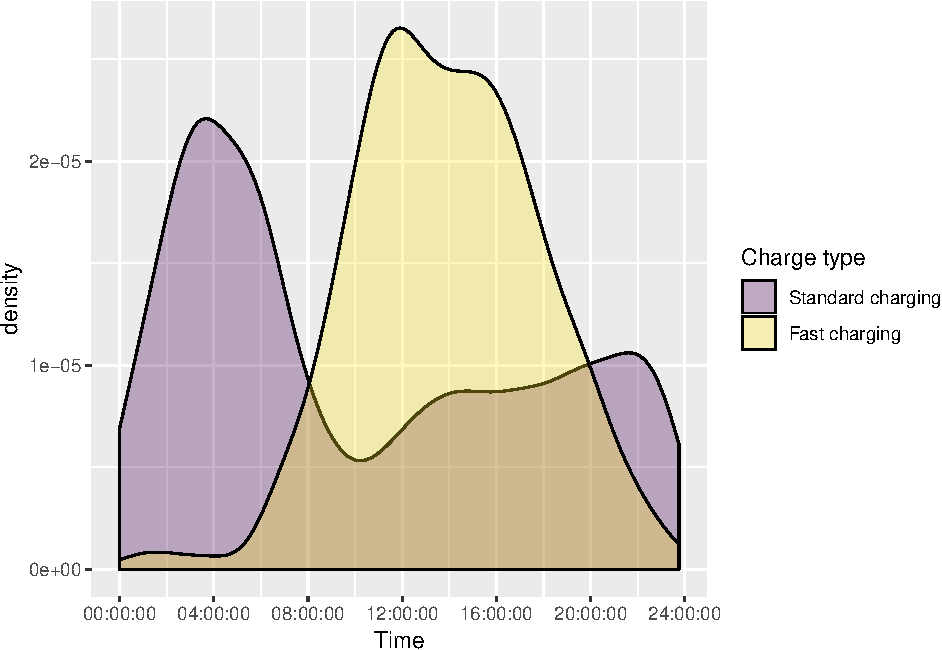
\includegraphics{EVBB_SummaryReport_files/figure-latex/chargeEndsWeekday-1.pdf}
\caption{\label{fig:chargeEndsWeekday}Density plot of charging end times
during weekdays}
\end{figure}

\begin{Shaded}
\begin{Highlighting}[]
\NormalTok{p <-}\StringTok{ }\KeywordTok{ggplot}\NormalTok{(chargeEnds[chargeEnds}\OperatorTok{$}\NormalTok{weekday }\OperatorTok{==}\StringTok{ "Weekend"}\NormalTok{, ], }\KeywordTok{aes}\NormalTok{(}\DataTypeTok{x =}\NormalTok{ qHour, }\DataTypeTok{fill =}\NormalTok{ chargeType))  }\OperatorTok{+}
\StringTok{  }\KeywordTok{scale_colour_manual}\NormalTok{(}\DataTypeTok{values=}\NormalTok{cbbPalette)}\OperatorTok{+}
\StringTok{  }\KeywordTok{geom_density}\NormalTok{(}\DataTypeTok{alpha =} \FloatTok{0.3}\NormalTok{) }\OperatorTok{+}
\StringTok{  }\KeywordTok{facet_grid}\NormalTok{(}\OperatorTok{~}\NormalTok{weekday)}
\NormalTok{p }\OperatorTok{+}\StringTok{ }\KeywordTok{labs}\NormalTok{(}\DataTypeTok{x =} \StringTok{"Time"}\NormalTok{, }\DataTypeTok{fill =} \StringTok{"Charge type"}\NormalTok{)}
\end{Highlighting}
\end{Shaded}

\begin{figure}
\centering
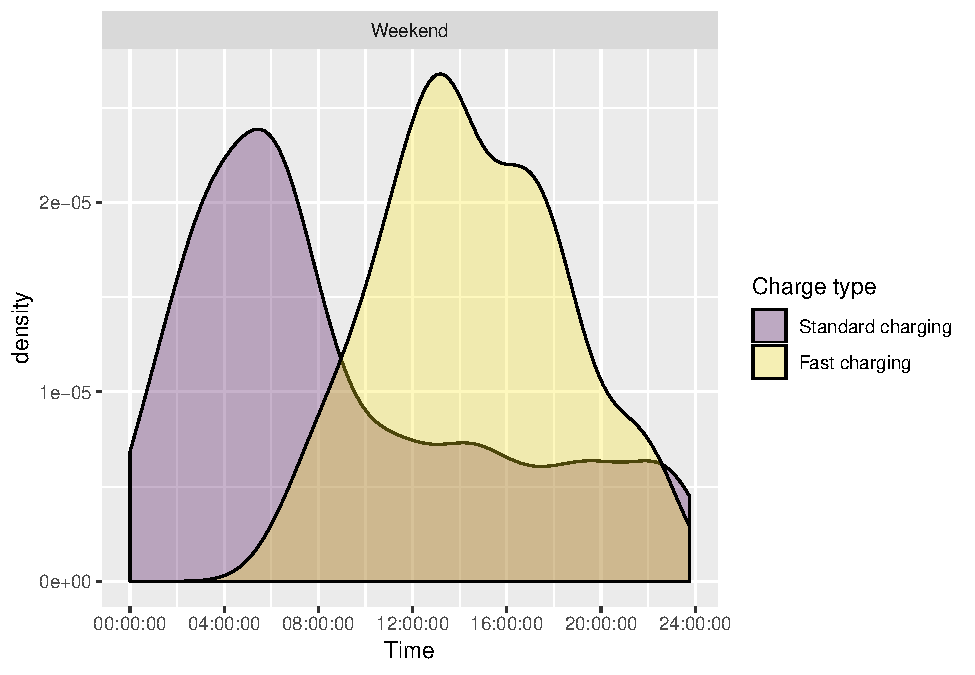
\includegraphics{EVBB_SummaryReport_files/figure-latex/chargeEndsWeekend-1.pdf}
\caption{\label{fig:chargeEndsWeekend}Density plot of charging end times
during weekends}
\end{figure}

At home charging events tended to begin at HH:MM during weekdays and
HH:MM at weekends. \emph{We can get ``Slow'' charging events rather than
``home''}

Standard charging has a noticeably different profile to charging
patterns for fast charges. It suggests that it is common for plug-in
vehicle owners to charge overnight at home, and perhaps use the more
powerful public chargepoints to top up during the day.

\begin{quote}
Discuss any other patterns
\end{quote}

\section{State of charge}\label{state-of-charge}

The duration of charging events (see Section \ref{duration}) suggests
that EVs may be `plugged in' at home (and elsewhere) for considerable
durations.

\begin{Shaded}
\begin{Highlighting}[]
\NormalTok{p <-}\StringTok{ }\KeywordTok{ggplot}\NormalTok{(}\DataTypeTok{data=}\NormalTok{chargeBegins, }\KeywordTok{aes}\NormalTok{(chargeBegins}\OperatorTok{$}\NormalTok{SoC_percent)) }\OperatorTok{+}\StringTok{ }\KeywordTok{geom_histogram}\NormalTok{(}\DataTypeTok{bins =} \DecValTok{10}\NormalTok{)}
\NormalTok{p }\OperatorTok{+}\StringTok{ }\KeywordTok{labs}\NormalTok{(}\DataTypeTok{x =} \StringTok{"State of charge when charging begins (%)"}\NormalTok{)}
\end{Highlighting}
\end{Shaded}

\begin{verbatim}
## Warning: Removed 1 rows containing non-finite values (stat_bin).
\end{verbatim}

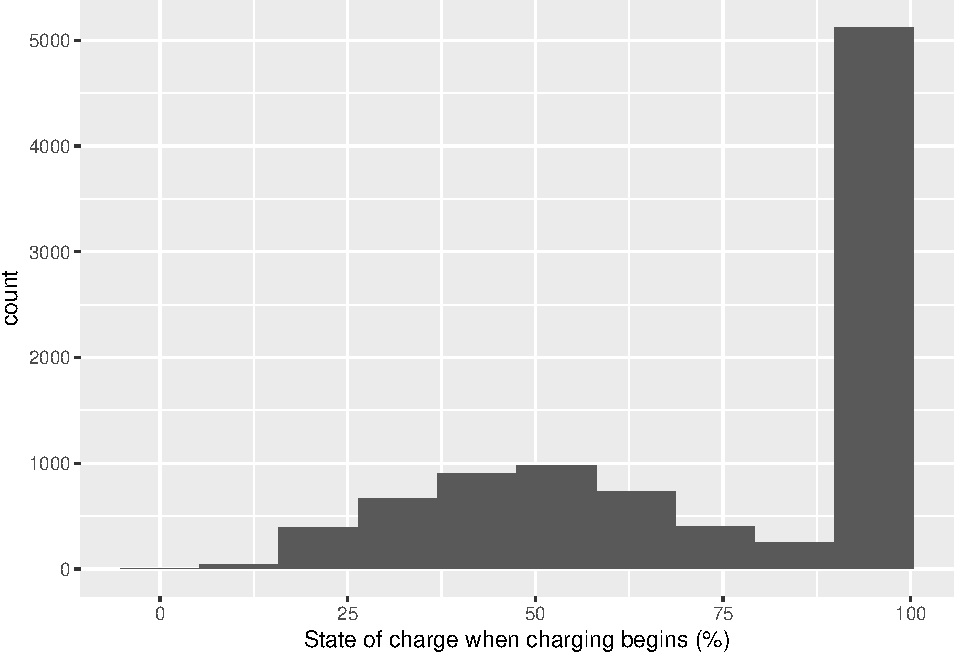
\includegraphics{EVBB_SummaryReport_files/figure-latex/value of state of charge at beginning of charge-1.pdf}

\begin{Shaded}
\begin{Highlighting}[]
\KeywordTok{ggsave}\NormalTok{(}\StringTok{"~/EVBB/plots/SOC_when_charging_begins.png"}\NormalTok{)}
\end{Highlighting}
\end{Shaded}

\begin{verbatim}
## Saving 6.5 x 4.5 in image
\end{verbatim}

\begin{verbatim}
## Warning: Removed 1 rows containing non-finite values (stat_bin).
\end{verbatim}

Fig: Distribution of state of charge when evening charge event starts
`at home' (histogram (or joy plot) by day of week)
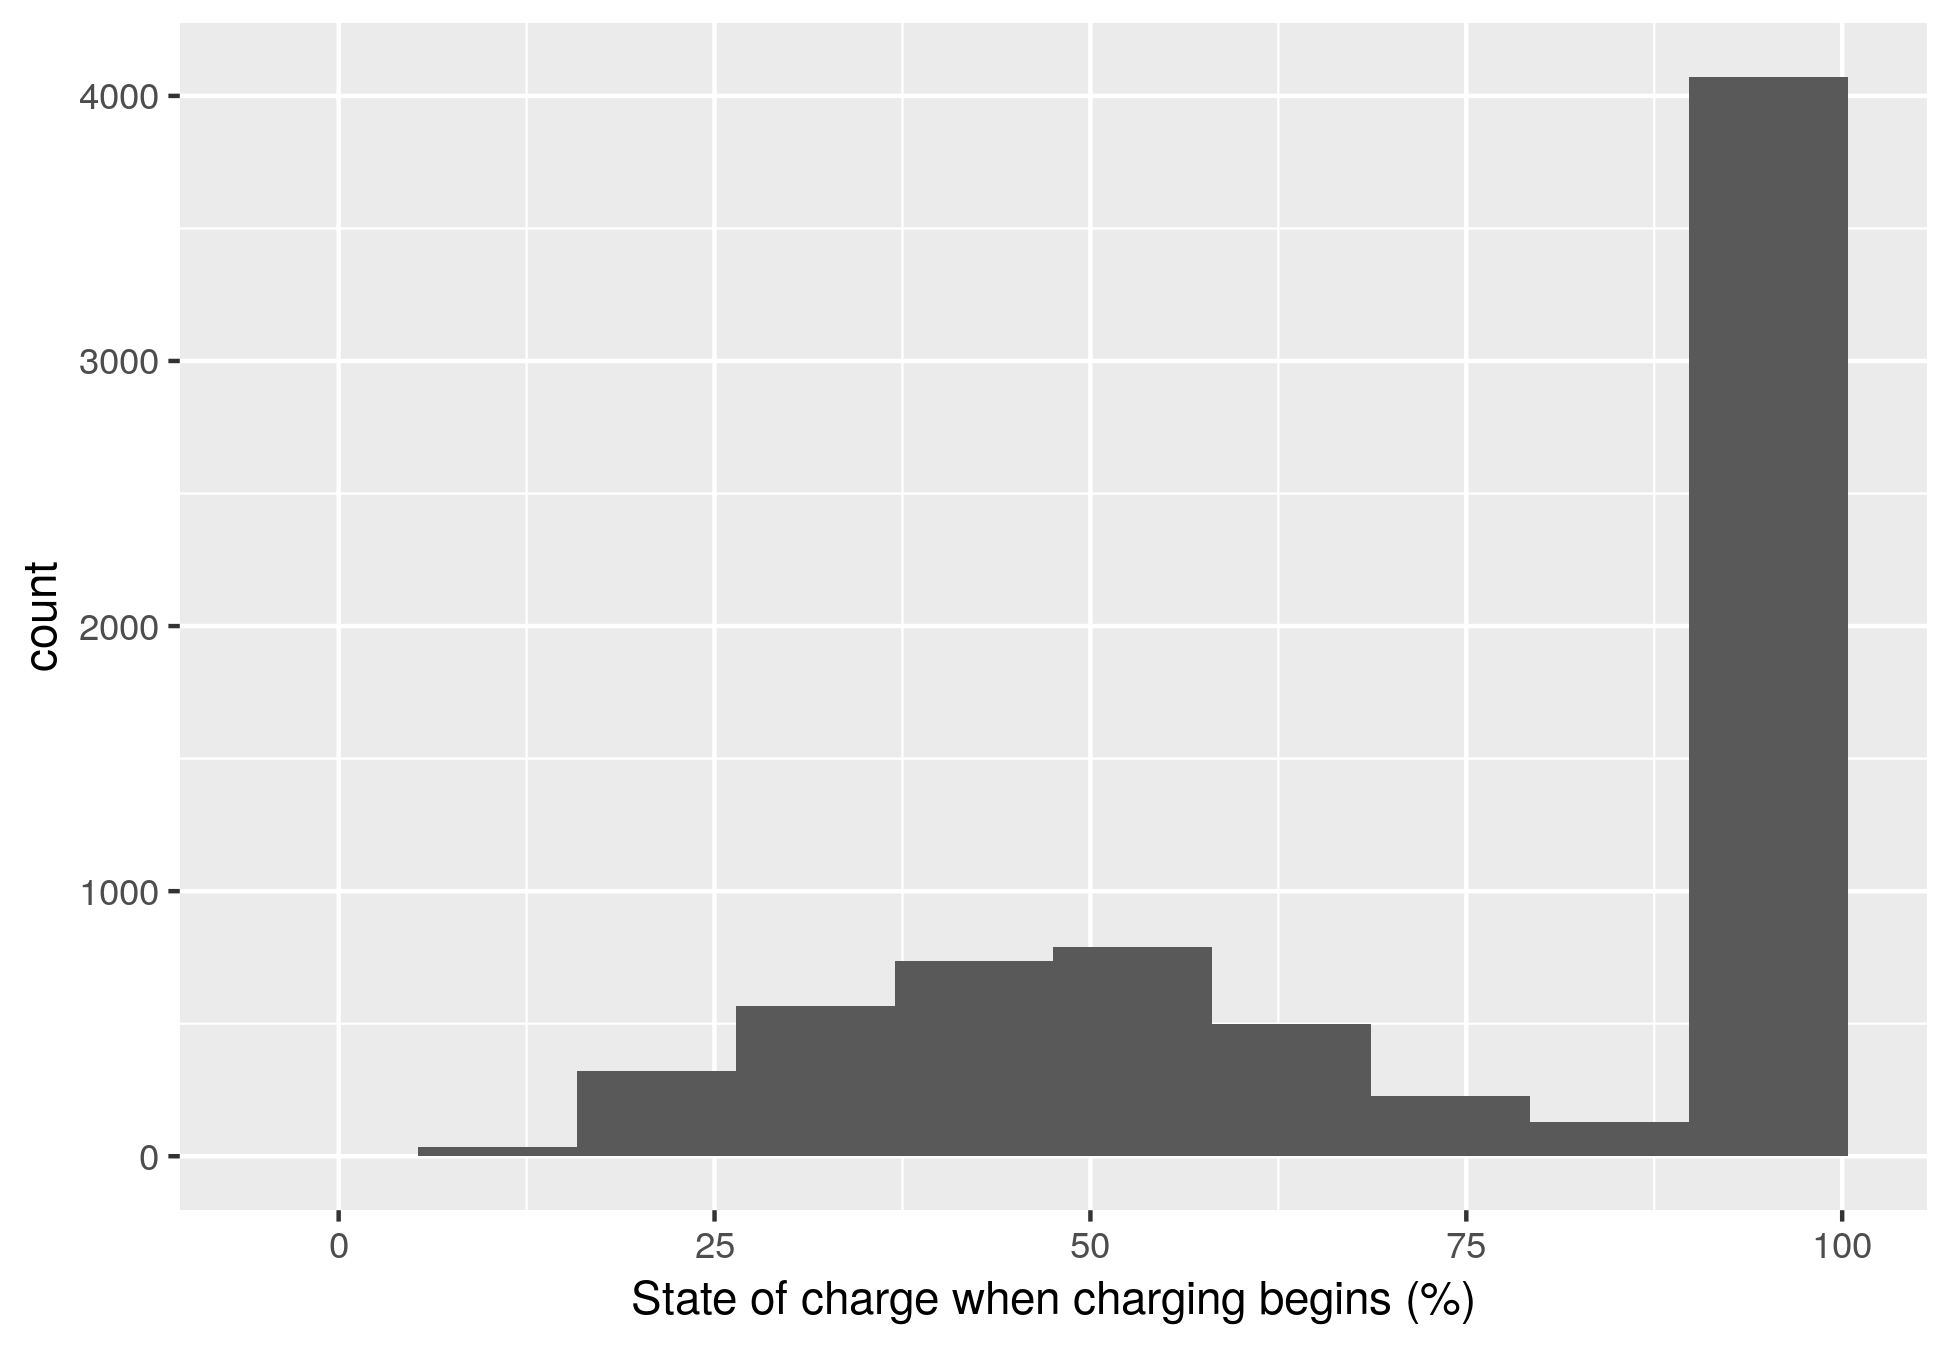
\includegraphics{~/EVBB/plots/SOC_when_charging_begins.png}

The figure shows that many vehicles arrive home with greater than 50\%
charge remaining and would therefore be able to transfer energy to the
home during the evening grid peak as a form of demand response.

Fig: Mean state of battery charge at the first `at home' charging
observation by hour and day of the week \emph{No ``at home'' data with
SOC}

\begin{quote}
should show the timing of `coming home' battery state?
\end{quote}

Fig: Distribution of duration of charge events starting `at home' in the
evening (by day of the week) \emph{Duration difficult to accurately
determine without date due to charging occurring through the night}

The figure shows that vehicles may then be available for further demand
response and/or re-charging for up to XX hours from this point.

\begin{quote}
Discuss any other patterns
\end{quote}


\end{document}
